%!TEX root = ../TAMUTemplate.tex
%%%%%%%%%%%%%%%%%%%%%%%%%%%%%%%%%%%%%%%%%%%%%%%%%%%
%
%  New template code for TAMU Theses and Dissertations starting Fall 2016.
%
%  Author: Sean Zachary Roberson
%    Version 3.16.09
%  Last updated 9/12/2016
%
%%%%%%%%%%%%%%%%%%%%%%%%%%%%%%%%%%%%%%%%%%%%%%%%%%%

%%%%%%%%%%%%%%%%%%%%%%%%%%%%%%%%%%%%%%%%%%%%%%%%%%%%%%%%%%%%%%%%%%%%%%%
%%%                           SECTION II
%%%%%%%%%%%%%%%%%%%%%%%%%%%%%%%%%%%%%%%%%%%%%%%%%%%%%%%%%%%%%%%%%%%%%%

\chapter{\texorpdfstring{\uppercase {Theoretical Framework}}{Theoretical Framework}}
\label{ch:theoretical_framework}

Since the mid-1970s, the Standard Model (SM) of particle physics has been the leading theory describing three of the four known fundamental forces (not including gravity) as well as classifying all of the known elementary particles.
Even during it's formative years, the SM's success at predicting new particles (i.e. the top quark in 1995) and describing the properties of known particles (i.e. $W^{\pm}$ to $Z^{0}$ mass ratio) was undeniable.
The model's roots can be traced back to 1930 when Herman Weyl was able to describe electromagnetism as a local symmetry represented by the Lie group $U\left(1\right)$~\cite{Weyl1929}.
In 1954 Yang and Mills created a theory which tried to extend the idea of gauge theory to non-abelian groups~\cite{PhysRev.96.191}.
This laid the ground work for Sheldon Glashow to combine the electromagnetic and weak interactions in 1961~\cite{GLASHOW1961579}.
This combined interaction is described by the $SU\left(2\right){\times}U\left(1\right)$ group.
In 1967 Steven Weinberg and Abdus Salam~\cite{PhysRevLett.19.1264,salam1968} continued this work by adding in the Higgs mechanism first proposed by Robert Brout and Francois Englert~\cite{PhysRevLett.13.321}, Peter Higgs~\cite{PhysRevLett.13.508,Higgs:1966ev}, and Gerald Guralnik, Carl. R. Hagen, and Tom Kibble~\cite{PhysRevLett.13.585,Kibble:1967sv}.
Although all of these theorist contributed to this advancement, the mechanism eventually became known as the Brout-Englert-Higgs (BEH) mechanism.
The model entered its current form around 1964 with the introduction of the strong force and quantum chromodynamics (QCD)~\cite{Neeman:1961jhl,GellMann:1962xb,GellMann:1964nj,Zweig:1981pd,Fritzsch:1972jv}.
The initial theory by Gell-Man and Zweig only included the up, down, and strange quarks and was incomplete until the introduction of the color charge by Greenberg~\cite{PhysRevLett.13.598}.
The full theory is described by the symmetry group
\begin{equation}\label{eq:standard_model_symmetry_group}
SU\left(3\right)_{C}{\otimes}SU\left(2\right)_{L}{\otimes}U\left(1\right)_{Y}
\end{equation}
where $SU\left(2\right)_{L}{\otimes}U\left(1\right)_{Y}$ is the electroweak (EW) symmetry group describing both the electromagnetic and weak interactions and $SU\left(3\right)_{C}$ is the symmetry group describing the strong interaction~\cite{Burgess2007,Aitchison2012}.

The rest of this chapter will discuss the standard model, both its structure and some of its mathematical underpinnings, in more detail.
Section~\ref{sec:standard_model} will introduce the particle content of the SM.
The QFTs that govern the SM interactions will be discussed in sections~\ref{sec:QED} to~\ref{sec:higgs_mechanism}.
In section~\ref{sec:BSM} we will briefly reference how Higgs physics can relate to physics beyond the SM.
More information about the history of the standard model can be found in appendix~\ref{appendix:standard_model_history}.

\section{The Standard Model}
\label{sec:standard_model}

The standard model is a locally gauge-invariant quantum field theory (QFT) in four-dimensional Minkowski space~\cite{Burgess2007,Barnes2010}.
The structure and particle content of the SM can be found in fig~\ref{fig:standard_model}.
The SM is composed of 12 fermions, the particles that make up matter, and 4 gauge bosons, the force-carrying particles which mediate the electromagnetic, weak, and strong interactions.
On its own, the basic symmetries of the standard model require that the gauge bosons (W$^\pm$,Z,$\gamma$,gluons) be massless.
However, we know that this is not true as experiments have shown that the $W$ and $Z$ bosons have quite a large mass.
The aforementioned Higgs mechanism takes care of this by spontaneously breaking the electroweak symmetry, giving mass to the quarks, the leptons, and the $W$ and $Z$ bosons~\cite{PhysRevLett.19.1264,salam1968,Dawson:1998yi}.

\begin{figure}[!hbt]
	%\scalebox{.45}{\input{StandardModel}}
	\centering
	\resizebox{0.95\textwidth}{!}{\input{StandardModel_CERNWebfest2012}}
	\caption{The Standard Model of particle physics. The model includes three generations of matter particles (leptons and quarks) as well as the gauge and Higgs bosons. Included in this drawing are the particle names, symbols, masses, spin, electric charge, and color charge, if applicable.}
	\label{fig:standard_model}
\end{figure}

Fermions are particles which obey Fermi-Dirac statistics and the Pauli exclusion principle, meaning that no two fermions may occupy the same quantum state within a given quantum system.
These particles have half-integer spin, often denoted as spin-1/2 particles, which means that their intrinsic angular momentum is $\hbar/2$.
For every fermion $f$ in the SM there exists an anti-fermion $\bar{f}$, which has an identical mass, but opposite quantum numbers.
The fermions in the SM are separated into six leptons and six quarks with these further separated into 3 generations of pairs of particles.
Each subsequent generation is ostensibly a heavier version of the previous generation, with the same quantum numbers.\footnote{The neutrinos may have a different mass ordering.}

Each generation of lepton can be broken down into a charged and neutral lepton.
For instance, the first generation is composed of the electron (\Pe), with charge $-\Pe$, and the electron neutrino ($\Pgn_{e}$).
The second and third generations contain the muon (\Pmu) and tau (\Ptau) along with their associated neutrinos.
Although the SM specifies that the neutrinos are massless, experiments have shown that this is not true.
While their exact masses are still unknown, upper bounds have been places on these and can be seen in fig~\ref{fig:standard_model}.
Each generation of lepton has an associated quantum number, called the lepton number, defined as $L_{\ell}=n_{\ell}-n_{\bar{\ell}}$.
First generation leptons have quantum numbers $L_{e}=+1$ and $L_{\mu}=L_{\tau}=0$ while the second and third generations have value $+1$ for their associated lepton number and zero otherwise.
The antileptons have oppositely signed lepton numbers.
The lepton numbers are a conserved quantity in the SM, which means that only lepton-antilepton pairs can be created or destroyed.\
That being said, neutrino oscillations, the phenomena of neutrinos changing flavor from one generation to the next, has been observed~\cite{Maltoni:2004ei}.
While this violates the conservation of lepton numbers within a generation, the total lepton number $L{\equiv}L_{e}+L_{\mu}+L_{\tau}$ may still be conserved.
All leptons interact through the weak interaction, but only the charged leptons interact using the electromagnetic interaction.
Because leptons lack the color charge they do not interact using the strong force.

Like the leptons, the three generation of quarks can be broken into one up-type quark and one down-type quark, categories which gain their name through the content of the first generation containing the up (\cPqu) and down (\cPqd) quarks.
The second generation is made up of the charm (\cPqc) and strange (\cPqs) quarks while the third is made up of the top (\cPqt) and bottom (\cPqb) quarks.
The up-type quarks have fractional electric charge of $Q=+2e/3$ and the bottom-type quarks have electric charge $Q=-e/3$.
As in the case of the leptons, the quarks have an associated baryon quantum number, $B$.
This quantity is conserved in all SM interactions and no exception has every been seen.
This means that only quark-antiquark pairs may be created or destroyed and also results in the stability of the lightest baryon, the proton.
Baryon number is defined as $B=\frac{1}{3}\left(n_{q}-n_{\bar{q}}\right)$, where, for example, the baryon number for a quark is $+1/3$ and $-1/3$ for an antiquark.
Quarks may interact through the electromagnetic and weak interactions, but unlike the lepton, quarks can also interact via the strong force.
This is because quarks also have color charge, which can have three values referred to as red, green, or blue. 
Antiquarks may contain charges of anti-red, anti-green, or anti-blue.
In the SM colorless particles are forbidden from existing on their own, which means that individual quarks, often referred to as bare quarks, have never been seen in nature.
Instead, quarks are always found as constituents of bound states called hadrons.
This group of composite particles may be further divided into mesons, bound states of a quark-antiquark pair, and baryons, bound states of three quarks and antiquarks.
The hadrons contain quark and antiquark combinations such that the bound state is a color singlet, often referred to as being colorless.
Mesons contain color-anticolor pairs while baryons consist of red, green, and blue charged quarks.
The masses of the quarks are hard to measure due to their confinement in hadrons, however, global averages have been made.

So far the particle content of the SM has been introduced along with the various force carriers.
The next few sections will go into greater detail about the specifics of the particle-particle interactions.
It will be helpful to keep in mind figure~\ref{fig:sm-interactions}, which shows all of the leading order SM interactions.

\begin{figure}[!hbt]
	\begin{center}
		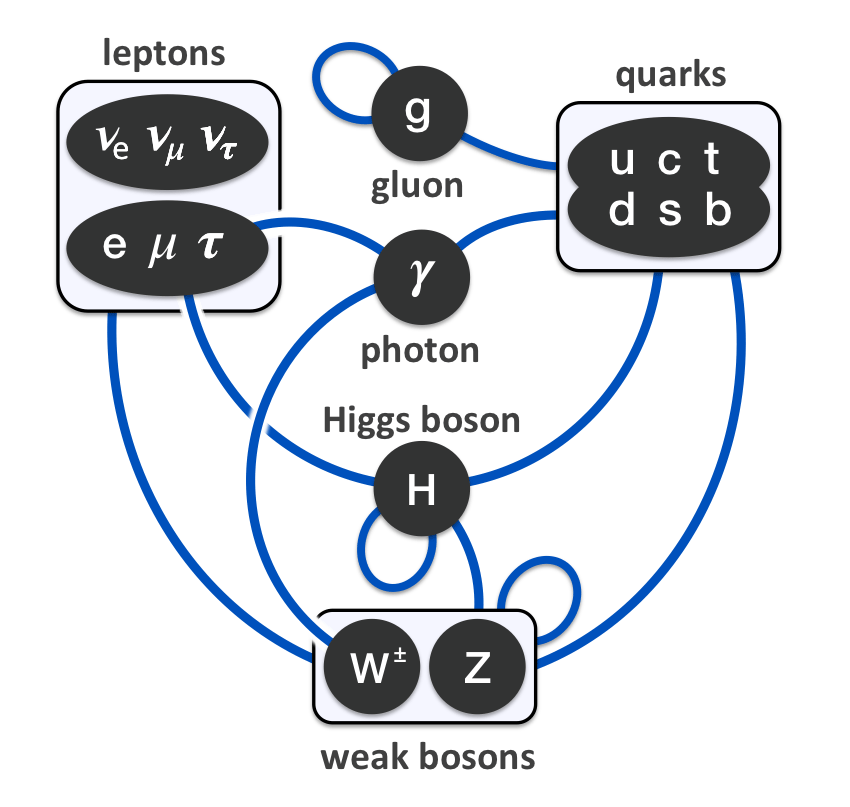
\includegraphics[width=0.95\textwidth]{figures/Chapter2/Elementary_particle_interactions_in_the_Standard_Model.png}
		\caption{A diagram illustrating the leading order interactions between particles in the standard model, including self-interactions~\cite{Drexler}.}
		\label{fig:sm-interactions}
	\end{center}
\end{figure}

\section{Quantum Electrodynamics \& the Electromagnetic Interaction}
\label{sec:QED}

Quantum electrodynamic (QED) is a quantum field theory which describes the dynamics of the electromagnetic interaction and corresponds to the $U_{EM}\left(1\right)$ group.
In a QFT, particles are represented by fields, which are in turn represented mathematically by Lagrangian densities $\mathcal{L}$.
QED was formulated to described the interactions of spin-1/2 particles, namely leptons and quarks.
Like a classical field theory, the dynamics of a quantum system are described by a Lagrangian.
QED is described by the Dirac Lagrangian density
\begin{equation}\label{eq:dirac_lagrangian_density}
\mathcal{L}=i\bar{\psi}\gamma^{\mu}\partial_{\mu}\psi-m\bar{\psi}\psi
\end{equation}
where $\psi$ a four-component column vector representing the wave function of a spin-1/2 particle\footnote{$\psi$ is a field known as a Dirac spinor.}, $\gamma^{\mu}$ are the four Dirac gamma matrices, $\bar{\psi}\equiv\psi^{\dagger}\gamma^{0}$, and $m$ is the mass of the particle.

In order for QED to be gauge invariant it must be invariant under both local and global gauge transformations.
Let there exist a global $U\left(1\right)$ transformation
\begin{equation}\label{eq:global_u1_transformation}
	\psi\rightarrow\psi'=e^{-i\alpha}\psi
\end{equation}
with constant $\alpha$.
Then $\psi$ in the Lagrangian~\ref{eq:dirac_lagrangian_density} can be replaced by equation~\ref{eq:global_u1_transformation}, which means that $\mathcal{L}\rightarrow\mathcal{L}'=\mathcal{L}$.
Therefore QED is invariant under this type of transformation.
If instead we have $\alpha\rightarrow\alpha\left(x\right)$ where $\alpha$ is allowed to vary as a function of space-time, then equation~\ref{eq:global_u1_transformation} becomes a local $U\left(1\right)$ transformation.
In this case equation~\ref{eq:dirac_lagrangian_density} becomes
\begin{equation}\label{eq:local_transformation}
	\mathcal{L}\rightarrow\mathcal{L}'=\mathcal{L}+\bar{\psi}\gamma^{\mu}\left(\partial_{\mu}\alpha\left(x\right)\right)\psi
\end{equation}
and is thus not invariant under the local transformation as is.
To return the gauge invariance we can replace the partial derivative in the Lagrangian density by a covariant derivative
\begin{equation}\label{eq:covariant_derivative}
	D_{\mu}=\partial_{\mu}+iqA_{\mu}
\end{equation}
, where $q=-e$ is the electron charge, in case of an electron, and $A_{\mu}$ is a new gauge field representing the photon, the mediator of electromagnetic interactions.
This new gauge field transforms as
\begin{equation}\label{eq:photon_transformation}
	A_{\mu}{\rightarrow}A_{\mu}'=A_{\mu}+\partial_{\mu}\chi\left(x\right)
\end{equation}
, where $\chi\left(x\right)$ is an arbitrary function of space-time.
When the transformation in equation~\ref{eq:global_u1_transformation} is made to a lepton field, the photon field transforms as in equation~\ref{eq:photon_transformation}, and $\chi\left(x\right)=\alpha\left(x\right)/q$, the covariant derivative transforms in the same way as $\psi\left(x\right)$, namely $D_{\mu}\psi\rightarrow\left(D_{\mu}\psi\right)'=e^{-i\alpha}D_{\mu}\psi$.
After the changes listed above, equation~\ref{eq:dirac_lagrangian_density} will take the locally gauge invariant form
\begin{equation}\label{eq:dirac_lagrangian_density_local_invariant}
	\mathcal{L}=\bar{\psi}\left(i\gamma^{\mu}D_{\mu}-m\right)\psi-\frac{1}{4}F^{\mu\nu}F_{\mu\nu}
\end{equation}
where
\begin{equation}\label{eq:electromagnetic_field_strength_tensor}
	F^{\mu\nu}=\left(\partial^{\mu}A^{\nu}-\partial^{\nu}A^{\mu}\right)
\end{equation}
is the electromagnetic field strength tensor.

Notice that in equation~\ref{eq:dirac_lagrangian_density_local_invariant} does not contain a $m^{2}A_{\mu}A^{\mu}$ term, which would be the mass of the gauge field.
This fits with experimental observations given that the photon is massless and thus the electromagnetic interaction has an infinite range.
Lagrangian~\ref{eq:dirac_lagrangian_density_local_invariant} does introduce lepton-photon interactions and does contain an $\ell^{+}\ell^{-}\gamma$ interaction and a term quadratic in the field strength tensor, which is the photon kinetic energy.
The complete QED Lagrangian can be created by generalizing to all leptons by $\psi\rightarrow\psi_{i}$ and summing over all leptons $i=e,\mu,\tau,u,d,c,s,t,b$ as in equation~\ref{eq:qed_lagrangian}.
\begin{equation}\label{eq:qed_lagrangian}
	\mathcal{L}=\sum_{i}\left[\bar{\psi}_{i}\left(i\gamma^{\mu}D_{\mu}-m_{i}\right)\psi_{i}\right]-\frac{1}{4}F_{\mu\nu}F^{\mu\nu}
\end{equation}

\section{Electroweak Interaction}
\label{sec:electroweak_interaction}

As mentioned in sec~\ref{ch:theoretical_framework}, the electromagnetic and weak interactions can be unified into a single, non-abelian gauge theory, work started by Yang \& Mills and then completed by Glashow, Weinberg, and Salam~\cite{Dawson:1998yi}.
In order to explain this unification, we will first work with a fermionic doublet representing and $SU\left(2\right)$ symmetry.
A doublet of Dirac fields can be represented as
\begin{equation}\label{eq:dirac_field_doublet}
	\psi=\doublet[r]{\psi_{1}\left(x\right)}{\psi_{2}\left(x\right)}
\end{equation}
The doublet will transform under the three dimensional rotation
\begin{equation}\label{eq:three_dimensional_rotation}
	\psi\rightarrow\exp\left<i\alpha^{i}\frac{\sigma_{i}}{2}\right>\psi
\end{equation}
This is again a global transformation, but note that by generalizing to higher order interaction we must use matrices instead of a local $\alpha\left(x\right)$ function to describe dynamics.
These matrices, $\sigma^{i}$, are the Pauli sigma matrices shown in equation~\ref{eq:pauli_sigma_matrices} and satisfy the identity $\sigma^{i}\sigma^{j}=\delta^{ij}+i\epsilon^{ijk}\sigma^{k}$ where $\epsilon^{ijk}=+1$ and where $\epsilon$ is an antisymmetric tensor.
\begin{equation}\label{eq:pauli_sigma_matrices}
	\sigma^{1}=\twoByTwo{0}{1}{1}{0},\text{ }\sigma^{2}=\twoByTwo{0}{-i}{i}{0},\text{ }\sigma^{3}=\twoByTwo{1}{0}{0}{-1}
\end{equation}

As in sec~\ref{sec:QED} we can turn equation~\ref{eq:three_dimensional_rotation} into a local transformation by having $\alpha\rightarrow\alpha^{i}\left(x\right)$ and thus
\begin{equation}
	\psi\left(x\right){\rightarrow}V\left(x\right)\psi\left(x\right)\text{, where }V\left(x\right)=\exp\left(i\alpha^{i}\left(x\right)\frac{\sigma^{i}}{2}\right)
\end{equation}
Still, the Lagrangian must be invariant under this transformation and in order to do this we introduce three vector fields $A_{\mu}^{i}\left(x\right)$, where $i=1,\;2,\;3$.
We once again use a covariant derivative
\begin{equation}
	D_{\mu}=\partial_{\mu}-igA_{\mu}^{i}\frac{\sigma^{i}}{2}
\end{equation}
, which means that the newly introduced fields transform as
\begin{equation}
	A_{\mu}^{i}\left(x\right)\frac{\sigma^{i}}{2}{\rightarrow}V\left(x\right)\left(A_{\mu}^{i}\left(x\right)\frac{\sigma^{i}}{2}+\frac{i}{g}\partial_{\mu}\right)V^{\dagger}\left(x\right)
\end{equation}
Unfortunately, this transformation is not trivial to calculate given that the Pauli matrices do not commute.
By assuming infinitesimally small transformations and expanding $V\left(x\right)$ to first order in $\alpha$ we obtain the simpler form
\begin{equation}
A_{\mu}^{i}\frac{\sigma^{i}}{2}{\rightarrow}A_{\mu}^{i}\frac{\sigma^{i}}{2}+\frac{1}{g}\left(\partial_{\mu}\alpha^{i}\right)\frac{\sigma^{i}}{2}+i\left[\alpha^{i}\frac{\sigma^{i}}{2},A_{\mu}^{i}\frac{\sigma^{i}}{2}\right]+...
\end{equation}
With the above ingredients the covariant derivative will transform as
\begin{equation}
	D_{\mu}\psi{\rightarrow}\left(1+i\alpha^{i}\frac{\sigma^{i}}{2}\right)D_{\mu}\psi
\end{equation}
and the field strength tensor will be
\begin{equation}
	F_{\mu\nu}^{i}=\partial_{\mu}A_{\nu}^{i}-\partial_{\nu}A_{\mu}^{i}+g\epsilon^{ijk}A_{\mu}^{j}A_{\nu}^{k}
\end{equation}
Given all of the above, the Yang-Mills Lagrangian will be
\begin{equation}\label{eq:yang_mills_lagrangian}
	\mathcal{L}=-\frac{1}{4}\left(F_{\mu\nu}^{i}\right)^{2}+\bar{\psi}\left(i\gamma^{\mu}\partial_{\mu}-igA_{\mu}^{i}\frac{\sigma^{i}}{2}\right)\psi
\end{equation}

Given the above process from Yang-Mills theory, we can now show how to obtain the electroweak interaction, which is based on a local $SU\left(2\right)_{L}{\times}U\left(1\right)_{Y}$ gauge symmetry. 
This process will follow what was done in section~\ref{sec:QED} in that requiring a local invariance will lead to the introduction of new gauge fields and determine their interactions.
It is also important to note that SM fermions can be grouped based on their chirality, which is a fundamental property of a particle and describes how the particles wave function will behave under rotation.
Spin-1/2 particles will pick up a minus sign under a $2\pi$ rotation, but left-chiral (left-handed) particles will go one way around the complex plane while right-chiral (right-handed) particles will go the opposite direction.
In the SM, the left-handed up- and down-type quarks form a weak doublet $q_{L}$ and the left-handed charged leptons and neutrinos form a separate weak doublet $\ell_{L}$.
The right-handed particles form weak singlets, but right-handed neutrinos and left-handed antineutrinos don't exist in the SM.

Given the prerequisites, an explanation of electroweak unification can now be made.
This explanation will start by using the first generation of leptons as an example, but will then generalize to more particles.
The SM contains an $SU\left(2\right)$ doublet of the left-handed components of the electron neutrino and electron.
The $SU\left(2\right)$ invariant right handed component of the electron is placed in a singlet.
\begin{equation}
	L_{e}=\doublet[r]{\nu_{L}}{e_{L}},\text{ }e_{R}
\end{equation}

The kinetic energy term of electroweak Lagrangian for the first generation leptons takes the form
\begin{equation}\label{eq:ew_kinetic_term_lagrangian}
	\mathcal{L}_{KE}^{e}=L_{e}^{\dagger}\tilde{\sigma}^{\mu}i\partial_{\mu}L_{e}+e_{R}^{\dagger}\sigma^{\mu}i\partial_{\mu}e_{R}
\end{equation}
where $\sigma=\left(\sigma^{0},\sigma^{1},\sigma^{2},\sigma^{3}\right)$, $\tilde{\sigma}=\left(\sigma^{0},-\sigma^{1},-\sigma^{2},-\sigma^{3}\right)$, $\sigma^{0}$ is an identity matrix, and $\sigma^{i}$ are again the Pauli matrices.
Equation~\ref{eq:ew_kinetic_term_lagrangian} is invariant under the global $SU\left(2\right)_{L}{\times}U\left(1\right)_{Y}$ transformation given by
\begin{equation}
	L{\rightarrow}L'=e^{i\theta}UL\hspace{1em}\forall\hspace{1em}\theta\in\mathbb{R}
\end{equation}
\begin{equation}
	e_{R}{\rightarrow}e_{R}'=e^{2i\theta}e_{R}\hspace{1em}\forall\hspace{1em}\theta\in\mathbb{R}
\end{equation}
where $U=e^{-i\alpha^{k}\sigma^{k}}$ and $\alpha^{k}$ is a real number.
However, the Lagrangian is not invariant under a local $SU\left(2\right)_{L}{\times}U\left(1\right)_{Y}$ transformation where $\theta$ and $\alpha^{k}$ are allowed to vary as a function of space-time.

To make Lagrangian~\ref{eq:ew_kinetic_term_lagrangian} invariant we introduce a $U\left(1\right)$ gauge field $B_{\mu}\left(x\right)$ and three $SU\left(2\right)$ gauge fields $W_{\mu}\left(x\right)=W_{\mu}^{k}\left(x\right)\sigma_{k}$ which transform as
\begin{equation}
	B_{\mu}\left(x\right){\rightarrow}B_{\mu}'\left(x\right)=B_{\mu}\left(x\right)+\frac{2}{g_{1}}\partial_{\mu}\theta\left(x\right)
\end{equation}
\begin{equation}
	W_{\mu}\left(x\right){\rightarrow}W_{\mu}'\left(x\right)=U\left(x\right)W_{\mu}\left(x\right)U^{\dagger}\left(x\right)+\frac{2i}{g_{2}}\left(\partial_{\mu}U\left(x\right)\right)U^{\dagger}\left(x\right)
\end{equation}
where $g_{1}$ and $g_{2}$ are dimensionless coupling strengths of the interactions.
The covariant derivatives are then
\begin{equation}
	D_{\mu}L_{e}=\left(\partial_{\mu}+i\frac{g_{1}}{2}YB_{\mu}+i\frac{g_{2}}{2}YW_{\mu}\right)L_{e}
\end{equation}
\begin{equation}
	D_{\mu}e_{R}=\left(\partial_{\mu}+i\frac{g_{1}}{2}YB_{\mu}\right)e_{R}
\end{equation}
where $Y$ is the hypercharge operator.
The weak hypercharge can be calculated as $Y=2\left(Q-T_{3}\right)$, where $T_{3}$ is the third component of the weak isospin quantum number $T$.
A notable property of the weak interaction is that it only acts on particles with weak isospin $T$ and that $T_{3}$ is conserved in all interactions.
The SM gauge fields and their associated electric and hypercharge values can be found in table~\ref{tab:fermion_quantum_numbers}.
Combining the kinetic and gauge interaction terms of the Lagrangian yields
\begin{equation}\label{eq:electron_electroweak_lagrangian}
	\mathcal{L}=\mathcal{L}_{KE}+\mathcal{L}_{gauge}=L_{e}^{\dagger}\tilde{\sigma}^{\mu}iD_{\mu}L_{e}+e_{R}^{\dagger}\sigma^{\mu}iD_{\mu}e_{R}-\frac{1}{4}B_{\mu\nu}B^{\mu\nu}-\sum_{i=1}^{3}\frac{1}{4}W_{\mu\nu}^{i}W^{i\mu\nu}
\end{equation}
where $B_{\mu\nu}=\partial_{\mu}B_{\nu}-\partial_{\nu}B_{\mu}$ and $W_{\mu\nu}=\left[\partial_{\mu}+\left(i\frac{g_{2}}{2}\right)W_{\mu}\right]W_{\nu}-\left[\partial_{\nu}+\left(i\frac{g_{2}}{2}\right)W_{\nu}\right]W_{\mu}$ are the field strength tensors.
This Lagrangian, without any mass terms, is now locally invariant.
The addition of the mass terms and electroweak symmetry breaking (EWSB) will be covered in section~\ref{sec:higgs_mechanism}, but given that the mediators of the weak force are massive, its range is limited to about $10^{-18}\unit{m}$.

The observed electroweak gauge bosons are actually combinations of the $B$ and $W$ fields as shown in equation~\ref{eq:electroweak_bosons}
\begin{align}\label{eq:electroweak_bosons}
	W_{\mu}^{\pm}&=\frac{W_{\mu}^{1}{\mp}iW_{\mu}^{2}}{\sqrt{2}}\\
	Z_{\mu}&=\frac{g_{1}W_{\mu}^{3}-g_{2}B_{\mu}}{\sqrt{g_{1}^{2}+g_{2}^{2}}}&=W_{\mu}^{3}\cos\left(\theta_{W}\right)-B_{\mu}\sin\left(\theta_{W}\right)\\
	A_{\mu}&=\frac{g_{1}W_{\mu}^{3}+g_{2}B_{\mu}}{\sqrt{g_{1}^{2}+g_{2}^{2}}}&=W_{\mu}^{3}\sin\left(\theta_{W}\right)-B_{\mu}\cos\left(\theta_{W}\right)
\end{align}
, where $\theta_{W}$ is the Weinberg angle defined as $\sin\left(\theta_{W}\right)=g_{1}/\sqrt{g_{1}^{2}+g_{2}^{2}}$.
Note that $W_{1}$ and $W_{2}$ are electrically charged while $W_{3}$ and $B$ are electrically neutral.
Given equation~\ref{eq:electron_electroweak_lagrangian}, the $W^{\pm}$ will only couple to the left-handed doublets while the $Z$ and photon ($A$) will couple to both the left- and right-handed leptons in the SM.
Lagrangian~\ref{eq:electron_electroweak_lagrangian} can be generalized to include the other generations by appropriately summing over all leptons as in equation~\ref{eq:lepton_electroweak_lagrangian}.
\begin{equation}\label{eq:lepton_electroweak_lagrangian}
	\mathcal{L}^{\ell}=\sum_{leptons}\left(L_{e}^{\dagger}\tilde{\sigma}^{\mu}iD_{\mu}L_{e}+e_{R}^{\dagger}\sigma^{\mu}iD_{\mu}e_{R}\right)-\frac{1}{4}B_{\mu\nu}B^{\mu\nu}-\sum_{i=1}^{3}\frac{1}{4}W_{\mu\nu}^{i}W^{i\mu\nu}
\end{equation}

These ideas can be extended to the quarks by making a doublets out of the left-handed up- and down-type quarks and singlets out of the right handed components, as in~\ref{eq:ew_quark_extension}.
\begin{equation}\label{eq:ew_quark_extension}
	Q_{u}=\doublet[r]{u_{L}}{d_{L}},\text{ }u_{R},\text{ }d_{R}
\end{equation}
A similar kinetic component to the lepton Lagrangian in~\ref{eq:ew_kinetic_term_lagrangian} can also be formed
\begin{equation}\label{eq:ew_quark_kinetic_term_lagrangian}
	\mathcal{L}_{KE}^{quark}=Q_{u}^{\dagger}\tilde{\sigma}^{\mu}iD_{\mu}Q_{u}+u_{R}^{\dagger}\sigma^{\mu}iD_{\mu}u_{R}+d_{R}^{\dagger}\sigma^{\mu}iD_{\mu}d_{R}
\end{equation}
Once again the $W^{\pm}$ will only couple to the left-handed quark doublets while the $Z$ and photon will couple to both the left- and right-handed quarks.

\begin{table}[htbp]
	\caption{The quantum numbers of the SM fermions grouped by chirality and particle-type, independent of generation. The various particle-types in the SM are up-type quarks, down-type quarks, charged leptons, and neutrinos.}
	\centering
    \begin{tabular}{|l|l|r|r|r|r|r|}
\hline
      & \multicolumn{1}{c|}{Particle-Type} & \multicolumn{1}{c|}{$Q$} & \multicolumn{1}{c|}{$T_3$} & \multicolumn{1}{c|}{$Y$} & \multicolumn{1}{c|}{$B$} & \multicolumn{1}{c|}{$L$} \\
\hline
\multirow{3}{*}{Quarks}  
\rule{0pt}{24pt}         & $\cPq_L = \doublet[r]{\cPqu}{\cPqd}_L$ & $\doublet[r]{2/3}{-1/3}$ & $\doublet[r]{1/2}{-1/2}$ & $1/3$  & $1/3$ & 0 \\
                         & $\cPqu_R$                              & $2/3\hphantom{\bigg)}$   & $0\hphantom{\bigg)}$     & $4/3$  & $1/3$ & 0 \\
                         & $\cPqd_R$                              & $-1/3\hphantom{\bigg)}$  & $0\hphantom{\bigg)}$     & $-2/3$ & $1/3$ & 0 \\
\hline
\multirow{2}{*}{Leptons} 
\rule{0pt}{24pt}         & $\ell_L = \doublet[r]{\nu_{e}}{\Pe}_L$ & $\doublet[r]{0}{-1}$     & $\doublet[r]{1/2}{-1/2}$ & $-1$   & 0     & 1 \\
                         & $\Pe_R$                                & $-1\hphantom{\bigg)}$    & $0\hphantom{\bigg)}$     & $-2$   & 0     & 1 \\
\hline
    \end{tabular}
	\label{tab:fermion_quantum_numbers}
\end{table}

Adding equation~\ref{eq:ew_quark_kinetic_term_lagrangian} to equation~\ref{eq:lepton_electroweak_lagrangian} gives the full electroweak Lagrangian as
\begin{equation}\label{eq:electroweak_lagrangian}
	\mathcal{L}^{EW}=\mathcal{L}_{KE}^{lepton}+\mathcal{L}_{KE}^{quark}+\mathcal{L}_{gauge}
\end{equation}
This Lagrangian exhibits an invariance to the $U\left(1\right)$ transformation $L_{e}{\rightarrow}e^{i\alpha}L_{e},\text{ }e_{R}{\rightarrow}e^{i\alpha}e_{R}$, which leads to conservation of electron number.
There is a similar invariance to transformations using the muon and tau fields.
The Lagrangian is also invariant to another $U\left(1\right)$ transformation where all negatively (positively) charged fields are multiplied by $e^{i\alpha}$ ($e^{-i\alpha}$).
This invariance leads to the conservation of electric charge.
However, the electroweak Lagrangian is not invariant under charge conjugation or a parity transformation.
Charge is when the sign of all quantum numbers is changed or equivalently when all particles (antiparticles) are exchanged for antiparticles (particles).
Parity transformations occur when the sign of the spacial coordinates are flipped as in $\boldsymbol{r}{\rightarrow}-\boldsymbol{r}$.
Interactions mediated by the photon and Z boson, also known as neutral current interactions, are invariant under the combination of charge and parity transformations, known as CP invariance, but interactions mediated by the $W^{\pm}$ bosons in the quark sector are not invariant under a CP transformation~\cite{Kobayashi:1973fv}.

\section{Strong Interaction}
\label{sec:strong_interaction}

Quantum Chromodynamics (QCD) is the theory that described the interaction between quarks, the strong interaction, and is represented by a local $SU\left(3\right)_{C}$ gauge symmetry.
As mentioned in section~\ref{sec:standard_model}, quarks contain color charge (C) which comes in three varieties; red, green, and blue.
Only color neutral (colorless) hadrons are allowed in nature, which requires that a baryon contain equal parts of each color and that a meson contains a color-anticolor pair.
Because of this each quark is represented as a color triplet
\begin{equation}
	q_{u}=\triplet[r]{u_{r}}{u_{g}}{u_{b}}
\end{equation}
The mediator of the strong force, the electrically neutral gluon, must then contain two color charges in order to conserve color.
The eight known color combination for the gluon will represented by the eight gauge fields introduced below.

A QCD Lagrangian which is globally $SU\left(3\right)$ invariant can be represented as
\begin{equation}\label{eq:qcd_quark_lagrangian_global_invariant}
	\mathcal{L}_{QCD}^{q}=\sum_{i=1}^{6}\bar{q}_{i}i\gamma^{\mu}\partial_{\mu}q_{i}
\end{equation}
where $q_{i}$ represents one of the six quark flavors.
This Lagrangian will be invariant under a transformation of the form $q_{i}{\rightarrow}q_{i}'=Uq_{i}$ where $U$ is a member of $SU\left(3\right)$.
However, when using a local $SU\left(3\right)$ transformation where $U{\rightarrow}U\left(x\right)$, Lagrangian~\ref{eq:qcd_quark_lagrangian_global_invariant} is no longer invariant.
To return invariance, we must introduce eight gauge fields ($G_{\mu}\left(x\right)$), which represent the gluons, and the appropriate covariant derivative.
The transformation of the gauge fields and the covariant derivative will take the form
\begin{align}
	G_{\mu}{\rightarrow}G_{\mu}'&=UG_{\mu}U^{\dagger}+\frac{i}{g_{s}}\left(\partial_{\mu}U\right)U^{\dagger}\\
	D_{\mu}q_{i}&=\left(\partial_{\mu}+ig_{s}G_{\mu}\right)q_{i}
\end{align}
where $g_{s}$ is the dimensionless coupling strength of the color interaction and whose value can be seen in figure~\ref{fig:strong_coupling_constant} where $g_{s}=\alpha_{s}$.
The field strength tensor for QCD is
\begin{equation}
	G_{\mu\nu}=\partial_{\mu}G_{\nu}-\partial_{\nu}G_{\mu}+ig_{s}\left(G_{\mu}G_{\nu}-G_{\nu}G_{\mu}\right)
\end{equation}
and the locally $SU\left(3\right)$ gauge invariant QCD Lagrangian is given as
\begin{equation}\label{eq:qcd_quark_lagrangian}
	\mathcal{L}_{QCD}^{q}=\sum_{i=1}^{6}\left(\bar{q}_{i}i\gamma^{\mu}D_{\mu}q_{i}\right)-\frac{1}{4}\sum_{i=1}^{8}G_{\mu\nu}^{i}G^{i\mu\nu}
\end{equation}

\begin{figure}[!hbt]
	\begin{center}
		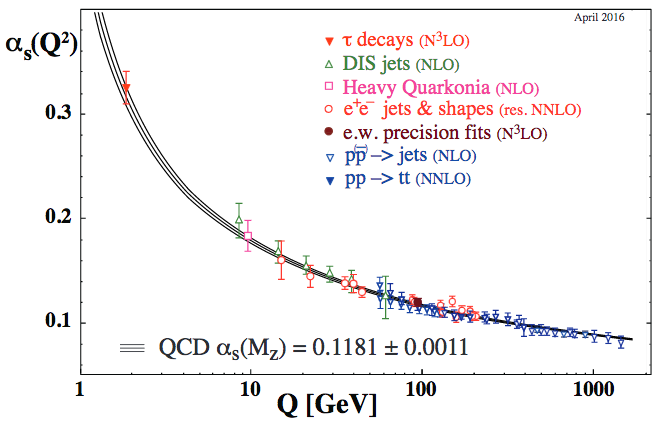
\includegraphics[width=0.95\textwidth]{figures/Chapter2/StrongCouplingConstant.png}
		\caption{Summary of measurements of $\alpha_{s}$ as a function of the energy scale $Q$. The respective degree of QCD perturbation theory used in the extraction of $\alpha_{s}$ is indicated in brackets (NLO: next-to-leading order; NNLO: next-to-next-to leading order; res. NNLO: NNLO matched with re-summed next-to-leading logs; N\textsuperscript{3}LO: next-to-NNLO). Figure and caption taken from~\cite{Olive:2016xmw}.}
		\label{fig:strong_coupling_constant}
	\end{center}
\end{figure}

There are a few interesting facts about the strong interaction which must be noted.
In contrast to the electroweak interaction C, P, and T are all conserved.
Additionally, the strong force has a range of about $10^{-15}\unit{m}$, which is enough to act on nucleons, i.e. protons and neutrons, to form atomic nuclei.
Lastly, QCD is a strongly coupled theory at low energies and large distance scales and weakly interacting at high energies and small distance scales.
Quarks are confined particles, meaning that the attractive force between them does not decrease as they move farther apart.
Instead the force decreases as the particles move closer and increases as they move farther apart, a behavior called asymptotic freedom~\cite{PhysRevLett.30.1343}.
When in the high energy regime the typical perturbative calculation can be made\footnote{The leading order (LO) terms can be calculated perturbatively. Corrections must be added to account for the next-to-leading order (NLO) effects, with further corrections for the next-to-next-to leading order (NNLO) effects, and so on.}, but in the low energy regime theorists must use more advanced techniques such as lattice gauge theory~\cite{Rothe2005}.

\section{Brout-Englert-Higgs Mechanism \& The Higgs Boson}
\label{sec:higgs_mechanism}

The EW and QCD Lagrangians covered in sections~\ref{sec:electroweak_interaction} and~\ref{sec:strong_interaction} contain no mass terms, which means the bosons within the SM should be massless.
However, we know from experiments at CERN that the $W^{\pm}$~\cite{ARNISON1983103} and $Z$~\cite{1983398} bosons do indeed have mass.
The method by which mass is added to the SM while maintaining the necessary gauge invariance is the BEH mechanism~\cite{PhysRevLett.13.321,PhysRevLett.13.508}.
This is accomplished by adding one or more complex scalar fields, the Higgs field(s), to the SM Lagrangian.
These fields will acquire a vacuum expectation value (vev) which will spontaneously break the symmetry of the Lagrangian.
The Goldstone theorem tells us that for every spontaneously broken continuous symmetry there will be a new massive scalar ``Goldstone'' boson.
So the number of Goldstone bosons will be equal to the number of broken generators of the symmetry group.
The massless standard model bosons then acquire mass by absorbing these Goldstone bosons.
So the number of massive SM bosons will be equal to the number of broken generators.

Remember from section~\ref{sec:electroweak_interaction} there are four massless electroweak gauge bosons, $W^{1}$, $W^{2}$, $W^{3}$, and $B^{0}$.
The experimentally observed bosons, however, are the massless photon ($\gamma$) and three massive bosons ($W^{\pm}$, $Z$).
We also know that the electric charge Q is conserved in electroweak interactions.
This means that the $SU\left(2\right)_{L}{\times}U\left(1\right)_{Y}$ electroweak theory is broken such that a new $U\left(1\right)_{EM}$ symmetry group is formed which corresponds to electromagnetism.
In order for three gauge bosons to acquire mass they must absorb three Goldstone bosons.
The simplest method to accomplish this is to introduce a complex, scalar $SU\left(2\right)$ doublet $\Phi$ with hypercharge $Y=1$.
\begin{equation}\label{eq:higgs_scalar_field}
	\Phi=\doublet[r]{\phi^{+}}{\phi^{0}}
\end{equation}
The part of the SM Lagrangian which includes the electroweak gauge bosons and the leptons can be written as
\begin{equation}
	\mathcal{L}_{SM}=-\frac{1}{4}W_{\mu\nu}^{a}W_{a}^{\mu\nu}-\frac{1}{4}B_{\mu\nu}B^{\mu\nu}+\bar{L}_{i}\left(iD_{\mu}\gamma^{\mu}\right)L_{i}+\bar{e}_{R,i}\left(iD_{\mu}\gamma^{\mu}\right)e_{R,i}
\end{equation}
where $i$ runs over the three generations, $\mu$ and $\nu$ are Lorentz indices, and $a$ runs over the generators in the gauge group.
The field strengths are given by
\begin{align}
	W_{\mu\nu}^{a}&=\partial_{\mu}W_{\nu}^{a}-\partial_{\nu}W_{\mu}^{a}+g_{2}\epsilon^{abc}W_{\mu}^{b}W_{\nu}^{c}\\
	B_{\mu\nu}&=\partial_{\mu}B_{\nu}-\partial_{\nu}B_{\mu}
\end{align}
and the covariant derivatives for the left- and right-handed leptons are
\begin{align}
	D_{\mu}L_{L}&=\left(\partial_{\mu}-ig_{2}T_{a}W_{\mu}^{a}-ig_{1}YB_{\mu}\right)L_{L}\\
	D_{\mu}e_{R}&=\left(\partial_{\mu}-ig_{1}YB_{\mu}\right)e_{R}
\end{align}
where $T_{a}$ are the generators of the $SU\left(2\right)_{L}$ gauge group and $g_{1}$, $g_{2}$ are the coupling constants for the electroweak interaction.

By adding the scalar field in equation~\ref{eq:higgs_scalar_field} we must add an additional scalar part to the Lagrangian
\begin{equation}\label{eq:higgs_scalar_lagrangian}
	\mathcal{L}_{S}=\left(D^{\mu}\Phi\right)^{\dagger}\left(D_{\mu}\Phi\right)-V\left(\Phi\right)
\end{equation}
where the first term is the kinetic term and the second term is the scalar potential, also known as the ``Mexican Hat'' potential.
While the form of the scalar potential is not known from first principles, we can make the assumption that it takes the simplest form possible which has the desired properties of spontaneous symmetry breaking and the ability to be renormalized
\begin{equation}
	V\left(\Phi\right)=\mu^{2}\Phi^{\dagger}\Phi+\lambda\left(\Phi^{\dagger}\Phi\right)^{2}
\end{equation}
The value of $\lambda$ must be positive in order for the vacuum to be stable.
The sign of $\mu^{2}$ specified one of two cases for the potential, both of which are illustrated in figure~\ref{fig:higgs_vev}. 
When $\mu^{2}>0$, the potential $V\left(\Phi\right)$ is always positive and has a minimum at
\begin{equation}
	\bra{0}\Phi\ket{0}\equiv\Phi_{0}=\doublet[r]{0}{0}
\end{equation}
where no spontaneous symmetry breaking can occur.
In contrast, when $\mu^{2}<0$ the potential takes its namesake ``Mexican hat'' shape with a minimum value not located at the origin.
In this case, the neutral component of the scalar field can acquire a vacuum expectation value (vev) $v$, a process known as electroweak symmetry breaking (EWSB).
\begin{equation}
	\bra{0}\Phi\ket{0}=\Phi_{0}=\frac{1}{\sqrt{2}}\doublet[r]{0}{v},\text{ }v=\sqrt{\frac{-\mu^{2}}{\lambda}}
\end{equation}
By only adding a vev to the neutral component of the scalar field electromagnetism is unbroken and the $U\left(1\right)_{EM}$ symmetry keeps a conserved electric charge of $Q=T_{3}+\frac{Y}{2}$.

\begin{figure}[hbt]
	\begin{center}
		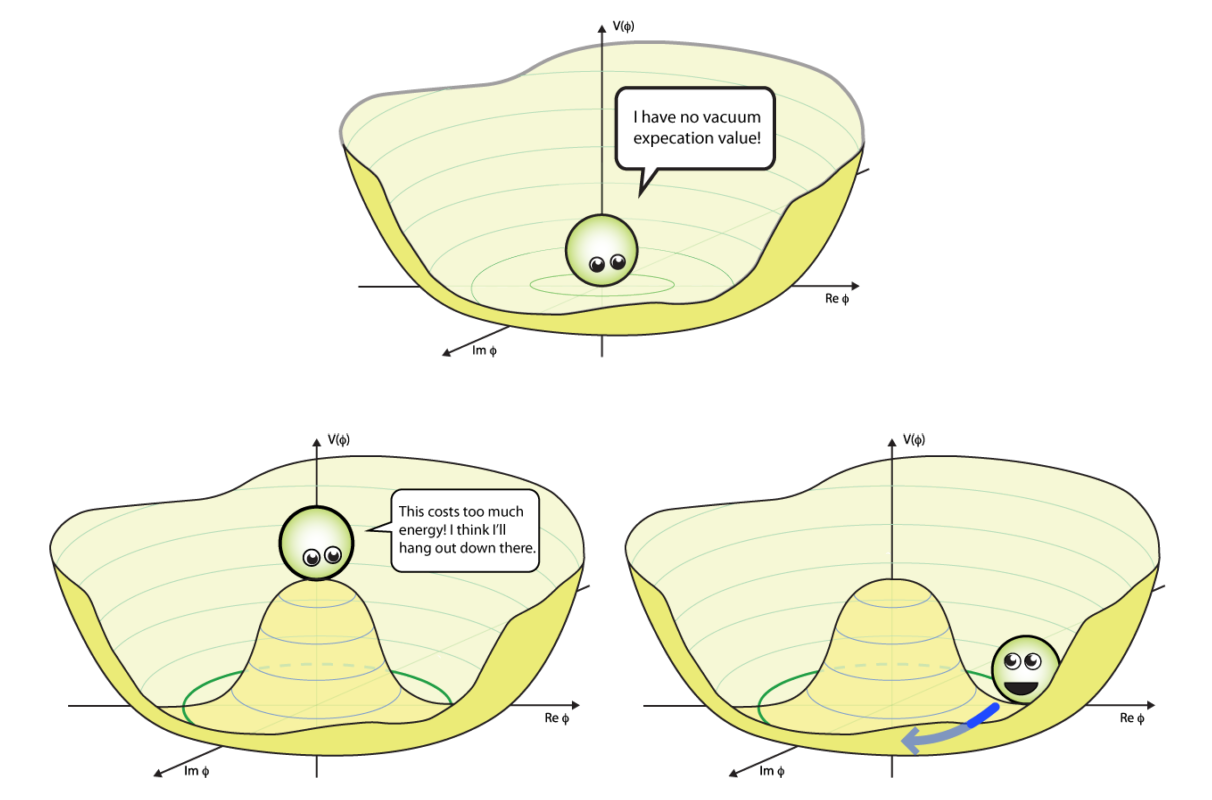
\includegraphics[width=0.95\textwidth]{figures/Chapter2/HiggsVEV.png}
		\caption{(Top) The scalar potential when $\mu^{2}>0$. In this case the potential will always be positive and its minimum value will be at the origin. The vacuum expectation value for this potential is zero. (Bottom) When $\mu^{2}<0$ the potential will take the shape of a ``Mexican Hat'' with its minimum value being in a degenerate ring around the origin. As soon as the scalar field has moves away from the origin and closer to the minimum the symmetry has been spontaneously broken and will acquire a non-zero vev. Because the scalar field picked a particular direction when falling towards the minimum, it is no longer invariant under a rotation~\cite{Tanedo}.}
		\label{fig:higgs_vev}
	\end{center}
\end{figure}

At this point we can expand the scalar field $\Phi$ around the minimum $\Phi_{0}$ to get
\begin{equation}\label{eq:scalar_field_with_higgs}
	\Phi\left(x\right)=\frac{1}{\sqrt{2}}\doublet[r]{0}{v+h\left(x\right)}
\end{equation}
where $h\left(x\right)$ is a new scalar field.
Next we insert this field into the kinetic part of the Lagrangian~\ref{eq:higgs_scalar_lagrangian} and redefine the gauge fields as
\begin{align}
	\label{eq:massive_W}W_{\mu}^{\pm}&=\frac{1}{\sqrt{2}}\left(W_{\mu}^{1}{\mp}iW_{\mu}^{2}\right)\\
	\label{eq:massive_Z}Z_{\mu}&=\frac{1}{\sqrt{g_{1}^{2}+g_{2}^{2}}}\left(g_{2}W_{\mu}^{3}-g_{1}B_{\mu}\right)\\
	\label{eq:massless_gamma}A_{\mu}&=\frac{1}{\sqrt{g_{1}^{2}+g_{2}^{2}}}\left(g_{2}W_{\mu}^{3}+g_{1}B_{\mu}\right)
\end{align}
which correspond to the observed gauge bosons.
After this the covariant derivative becomes
\begin{equation}
	|D_{\mu}\Phi|^{2}=\frac{1}{2}\left(\partial_{\mu}H\right)^{2}+\frac{1}{2}g_{2}^{2}\left(v+H\right)^{2}W_{\mu}^{+}W^{{\mu}-}+\frac{1}{8}\left(v+H\right)^{2}\left(g_{1}^{2}+g_{2}^{2}\right)Z_{\mu}Z^{\mu}
\end{equation}
From this we see that the photon $A_{\mu}$ remains massless, but that the mass terms for the $W$ and $Z$ bosons take the general forms $M_{W}^{2}W_{\mu}W^{\mu}$ and $\frac{1}{2}M_{Z}^{2}Z_{\mu}Z^{\mu}$ respectively.
Thus the masses of the electroweak gauge bosons are
\begin{align}
	\label{eq:mass_W}M_{W}&=\frac{1}{2}vg_{2}\\
	\label{eq:mass_Z}M_{Z}&=\frac{1}{2}v\sqrt{g_{1}^{2}+g_{2}^{2}}\\
	\label{eq:mass_gamma}M_{A}&=0
\end{align}
Three of the degrees of freedom from the scalar field, which would have been two charged and one neutral Goldstone boson, have been absorbed by the gauge bosons in order to give them mass.
These appear as \textit{flat} directions in the scalar potential.
There is one remaining degree of freedom, an oscillation in the radial direction, which corresponds to the neutral Higgs boson and can be seen in fig~\ref{fig:higgs_potential_radial} where the potential is concave.

\begin{figure}[hbt]
	\begin{center}
		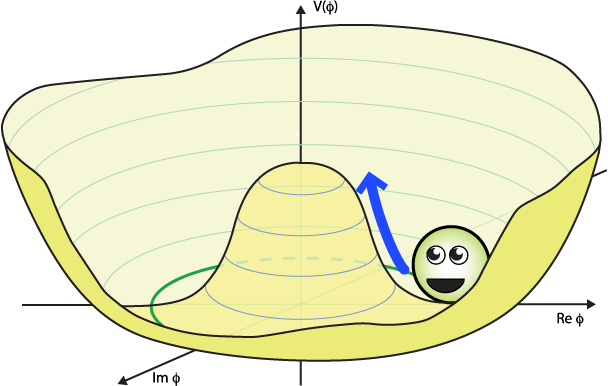
\includegraphics[width=0.95\textwidth]{figures/Chapter2/Higgs-Potential-radial.png}
		\caption{The Higgs boson corresponds to an oscillation of the scalar field in the radial direction~\cite{Tanedo}}
		\label{fig:higgs_potential_radial}
	\end{center}
\end{figure}

Several relationships can be formed between the various bosons.
The Weinberg angle also known as the weak mixing angle $\theta_{W}$, defined as $\sin\theta_{W}=\frac{g_{1}}{\sqrt{g_{1}^{2}+g_{2}^{2}}}$, can be used to describe the photon an Z as
\begin{align}
	A_{\mu}&=\cos\theta_{W}B_{\mu}+\sin\theta_{W}W_{\mu}^{3}\\
	Z_{\mu}&=-\sin\theta_{W}B_{\mu}+\cos\theta_{W}W_{\mu}^{3}
\end{align}
Equation~\ref{eq:weinber_wz} shows a relationship between the masses of the $W$ and $Z$ at tree level, which is one reason why measurements of their masses are so important.
\begin{equation}\label{eq:weinber_wz}
	\frac{M_{W}}{M_{Z}}=\frac{g_{2}}{\sqrt{g_{1}^{2}+g_{2}^{2}}}=\cos\theta_{W}
\end{equation}
There also exists a relationship between the coupling strength of the weak and electromagnetic interactions which makes use of the weak mixing angle,
\begin{equation}
	e=g_{2}\sin\theta_{W}
\end{equation}

By substituting equation~\ref{eq:scalar_field_with_higgs} into Lagrangian~\ref{eq:higgs_scalar_lagrangian}, using $v^{2}=-\frac{\mu^{2}}{\lambda}$, and looking at only the pieces involving the Higgs we can study the mass and couplings of the Higgs itself.
This section of the Lagrangian will take the form
\begin{equation}
	\mathcal{L}_{H}=\frac{1}{2}\left(\partial_{\mu}H\right)\left(\partial^{\mu}H\right)-{\lambda}v^{2}H^{2}-{\lambda}vH^{3}-\frac{\lambda}{4}H^{4}
\end{equation}
Since scalar masses have the general form $\frac{1}{2}m\phi^{2}$ we find that the Higgs boson mass is
\begin{equation}\label{eq:higgs_boson_mass}
	m_{H}=2{\lambda}v^{2}=-2\mu^{2},
\end{equation}
where $\lambda$, and thus the Higgs mass, needs to be determined experimentally.
We can also see that the Higgs couples to vector bosons, fermions, and itself, all interactions which are shown in figure~\ref{fig:higgs_boson_couplings}.

\begin{figure}[hbt]
    \centering
    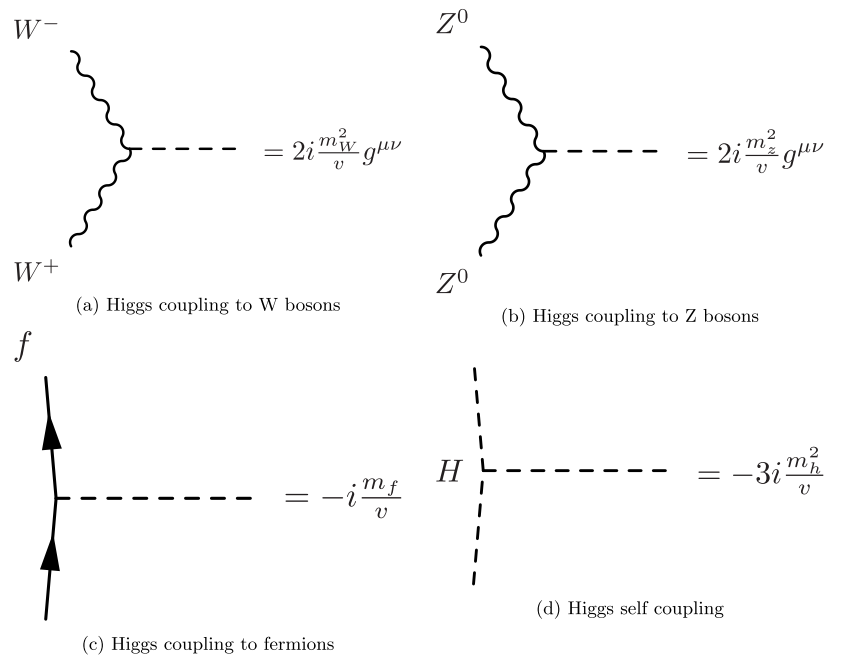
\includegraphics[width=0.95\textwidth]{\figpath/Chapter2/HiggsBosonCouplings.png}
    \caption{Tree level Feynman diagrams showing how the Higgs couples to vector bosons (a,b), fermions (c), and to itself (d).}
    \label{fig:higgs_boson_couplings}
\end{figure}

Besides having massive bosons, the SM also has a whole host of massive fermions.
These particles can be shown to acquire mass by adding Yukawa couplings between the fermion fields and the scalar field to the SM Lagrangian.
The part of the Lagrangian that corresponds to the first generation fermions is given by
\begin{equation}\label{eq:higgs_fermion_lagrangian}
	\mathcal{L}_{F}=-G_{e}\bar{L}{\Phi}e_{R}-G_{d}\bar{Q}{\Phi}d_{R}-G_{u}\bar{Q}\tilde{\Phi}u_{R}+h.c.
\end{equation}
where $\tilde{\Phi}=i\tau_{2}\Phi^{*}$ is the conjugate of $\Phi$ with negative hypercharge.
There are additional terms added to the full Lagrangian which correspond to the second and third generations which are not shown here.
By substituting equation~\ref{eq:scalar_field_with_higgs} into Lagrangian~\ref{eq:higgs_fermion_lagrangian} we find
\begin{align}
	%\phantom{\mathcal{L}_{F}}
	\begin{split}
		\mathcal{L}_{F}={}&-\frac{1}{\sqrt{2}}\left[G_{e}\rdoublet[r]{\bar{\nu}}{\bar{e}}_{L}\doublet[r]{0}{v+H}e_{R}+G_{d}\rdoublet[r]{\bar{u}}{\bar{d}}_{L}\doublet[r]{0}{v+h}d_{R}\right.\\
		&\qquad \left. +G_{u}\rdoublet[r]{\bar{u}}{\bar{d}}_{L}\doublet[r]{v+h}{0}u_{R}\right]+h.c.
	\end{split}\\
	\begin{split}
		={}&-\frac{1}{\sqrt{2}}\left(v+h\right)\left(G_{e}\bar{e}_{L}e_{R}+G_{d}\bar{d}_{L}d_{R}+G_{u}\bar{u}_{L}u_{R}\right)+h.c.
	\end{split}
\end{align}
where $h.c.$ is a placeholder for the hermitian conjugate terms.
The fermion masses take the form $m\bar{f}_{L}f_{R}+h.c.$, which means that the fermion masses for the first generation are
\begin{equation}
	m_{e}=\frac{G_{e}v}{\sqrt{2}},\hspace*{1cm}m_{u}=\frac{G_{u}v}{\sqrt{2}},\hspace*{1cm}m_{d}=\frac{G_{d}v}{\sqrt{2}}
\end{equation}
The second and third generations have similar mass terms.
Since there is no right handed neutrino in the SM the neutrinos that do exist remain massless.
As the coupling constants, G, and the fermion masses are not predicted by the SM they must be measured and added to the model.














\section{Higgs Production in a Proton-Proton Collider}
\label{sec:higgs_production}

The Higgs boson has several accessible productions mechanisms at a proton-proton collider.
Fig.~\ref{fig:HiggsProductionCrossSections} shows the 8\tev production cross sections for the five production modes at the LHC.
The production mode with the highest rate, by far, is the gluon-gluon fusion process shown in the blue curve, often abbreviated as \ggH.
Since gluons are massless so they can't couple directly to the Higgs boson.
Instead, this production mode proceeds through a fermion loop as shown in~\ref{fig:ggH}.
The Higgs couplings to fermions goes as $g_{H_{f\bar{f}}}=\frac{m_{f}}{v}$, where $v$ is the vacuum expectation value for the Higgs field, $v=\left(\sqrt{2}G_{F}\right)^{1/2}\approx\text{246}\gev$, where $G_{F}$ is the Fermi coupling determined by muon decay measurements~\cite{PDG}.
This means that the coupling is directly dependent upon the fermion mass and because of this the fermion loop in the gluon-gluon fusion diagram is dominated by top quarks, the heaviest of the fermions in the standard model.
The cross section for this production mechanism at \CM{8}\tev and assuming a 125\gev Higgs is
\begin{equation}
	\sigma_{\text{ggF}}=\text{19.27}_{-\text{7.8\%}}^{+\text{7.2\%}}\left(\text{QCD Scale Unc.}\right)_{-\text{6.9\%}}^{+\text{7.4\%}}\left(\text{PDF}+\alpha_{S}\text{ Unc.}\right)\pbinv
\end{equation}
where QCD Scale uncertainty refers to the next to next to leading order (NNLO) radiative corrections and $\text{PDF}+\alpha_{S}$ uncertainty refers to the uncertainties on the parton distribution function and strong coupling parameters.

\begin{figure}[!hbt]
  \centering
  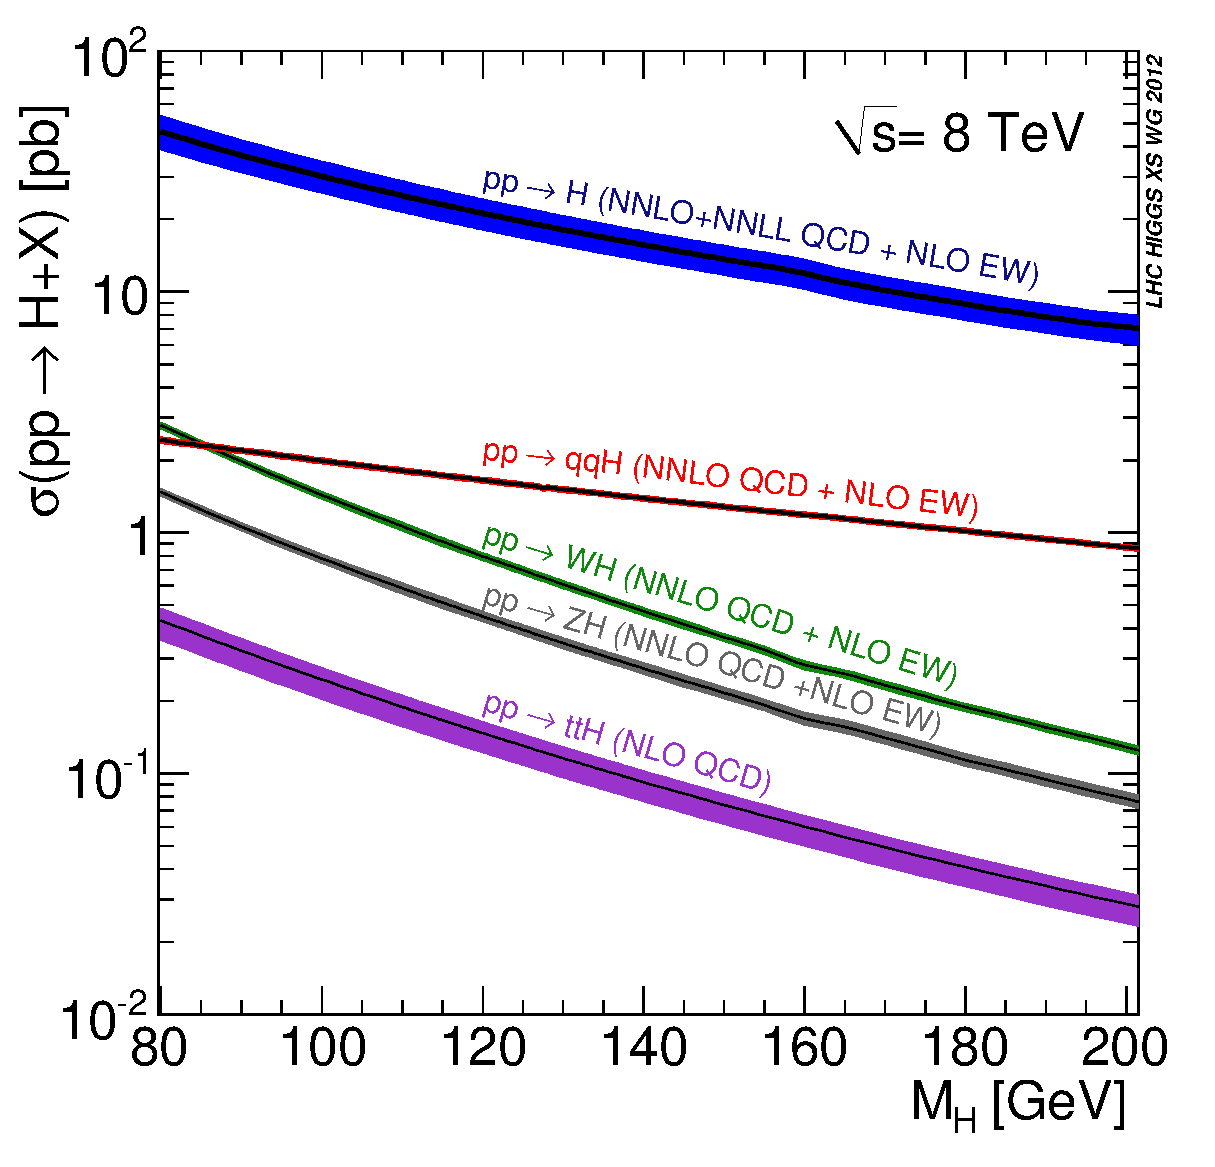
\includegraphics[width=0.95\textwidth]{\figpath/Chapter2/Higgs_XS_8TeV_LM200.eps}
  \caption{Higgs production cross-sections at the LHC for 8\TeV proton-proton collisions}
  \label{fig:HiggsProductionCrossSections}
\end{figure}

The production mechanism with the next highest cross section is the vector boson fusion (VBF) process (fig.~\ref{fig:qqH}) where either two oppositely charged \W bosons or two \Z bosons merge and produce a Higgs boson.
The final state particles for this process are those from the Higgs decay as well as the two initial quarks, which will preferentially be found in the forward regions of the detector, which is why this process is often abbreviated as \qqH.
The production cross section in this case is
\begin{equation}
	\sigma_{\text{VBF}}=\text{1.653}_{-\text{4.5\%}}^{+\text{4.5\%}}\left(\text{EW Unc.}\right)_{-\text{0.2\%}}^{+\text{0.2\%}}\left(\text{QCD Scale Unc.}\right)_{-\text{2.8\%}}^{+\text{2.6\%}}\left(\text{PDF}+\alpha_{S}\text{ Unc.}\right)\pbinv
\end{equation}
where the electroweak uncertainty is calculated at next to leading order (NLO).

The other processes found in fig.~\ref{fig:HiggsProductionCrossSections} can all be grouped as associated production mechanisms.
The Higgs is produced along with either a \Wpm boson, \Zz boson, or a \ttbar pair, often abbreviated as \WH, \ZH, or \ttH.
The first two cases, seen in fig.~\ref{fig:WH}, are also referred to as ``Higgsstralung'' because the Higgs can be seen as being radiated from the vector bosons, similar to how a photon is radiated by an electron during bremsstrahlung.
The latter case is seen in fig.~\ref{fig:ttH}.
The associated production cross sections are
\begin{align}
\begin{split}
	\sigma_{\text{WH}} &= \text{0.7046}_{-\text{1.0\%}}^{+\text{1.0\%}}\left(\text{QCD Scale Unc.}\right)_{-\text{2.3\%}}^{+\text{2.3\%}}\left(\text{PDF}+\alpha_{S}\text{ Unc.}\right)\pbinv \\
	\sigma_{\text{ZH}} &= \text{0.4153}_{-\text{3.1\%}}^{+\text{3.1\%}}\left(\text{QCD Scale Unc.}\right)_{-\text{2.5\%}}^{+\text{2.5\%}}\left(\text{PDF}+\alpha_{S}\text{ Unc.}\right)\pbinv \\
	\sigma_{\text{\ttbar{H}}} &= \text{0.1293}_{-\text{9.3\%}}^{+\text{3.8\%}}\left(\text{QCD Scale Unc.}\right)_{-\text{8.1\%}}^{+\text{8.1\%}}\left(\text{PDF}+\alpha_{S}\text{ Unc.}\right)\pbinv
\end{split}
\end{align}

\begin{figure}[bt]
  \centering
  \begin{subfigure}[t]{0.415\textwidth}
    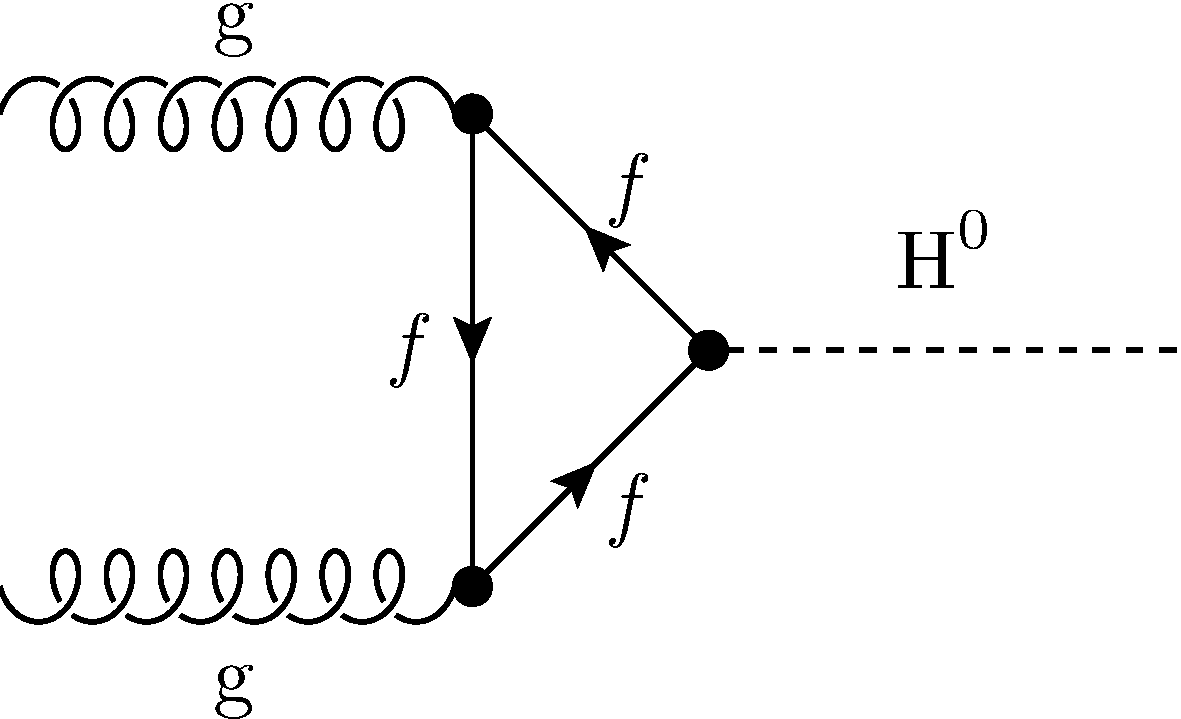
\includegraphics[width=\textwidth]{\figpath/FeynmanDiagramsPyFeyn/ggH.pdf}
    \caption{Gluon-gluon fusion}
    \label{fig:ggH}
  \end{subfigure}%
  \hspace{0.5cm}
  \begin{subfigure}[t]{0.415\textwidth}
    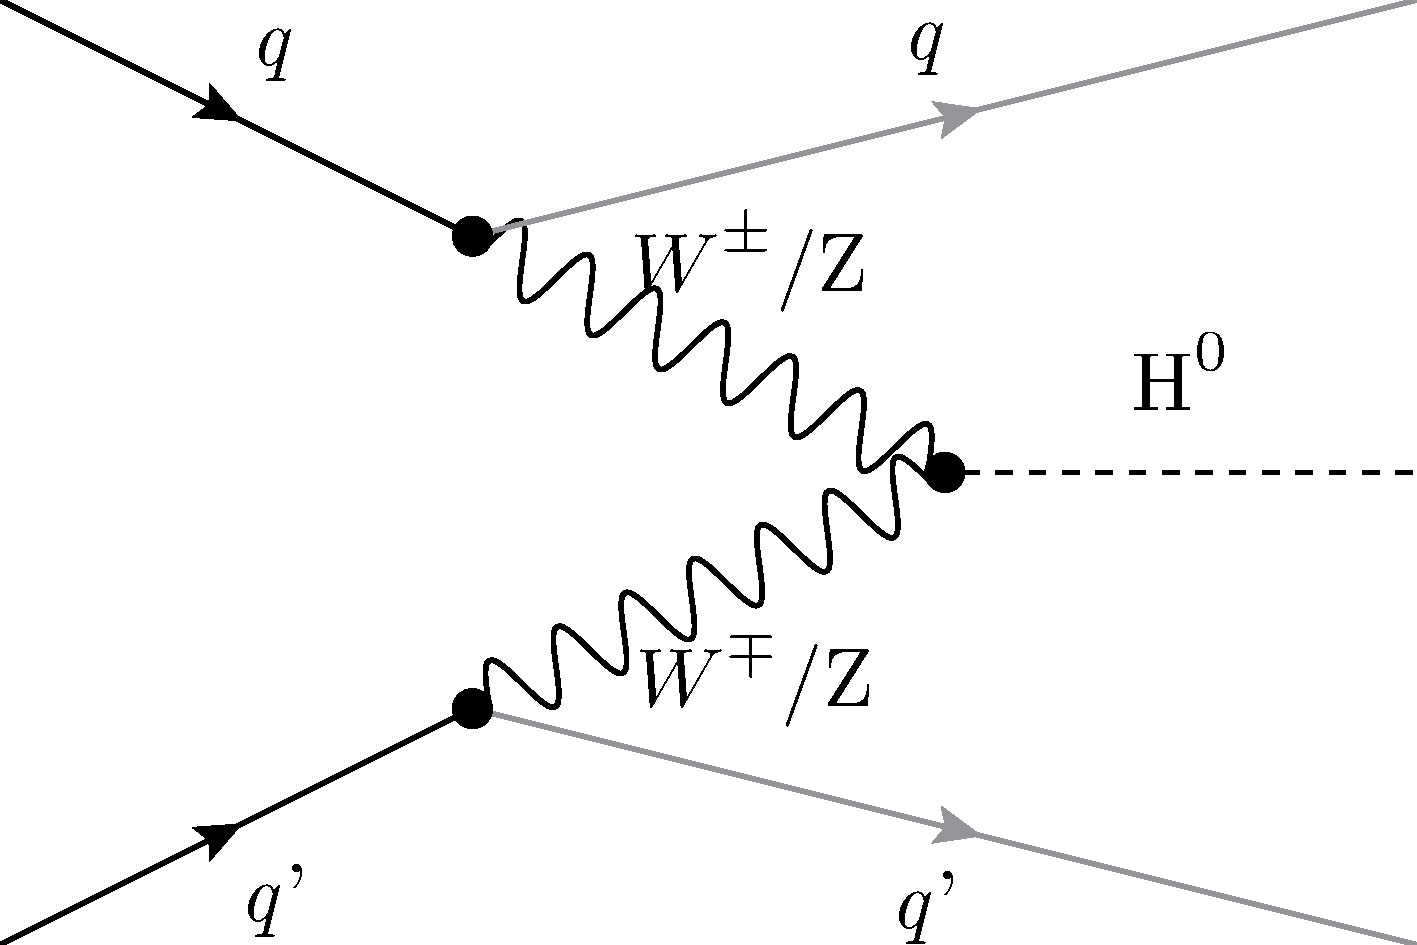
\includegraphics[width=\textwidth]{\figpath/FeynmanDiagramsPyFeyn/qqH.pdf}
    \caption{Vector boson fusion}
    \label{fig:qqH}
  \end{subfigure}

  \begin{subfigure}[t]{0.415\textwidth}
    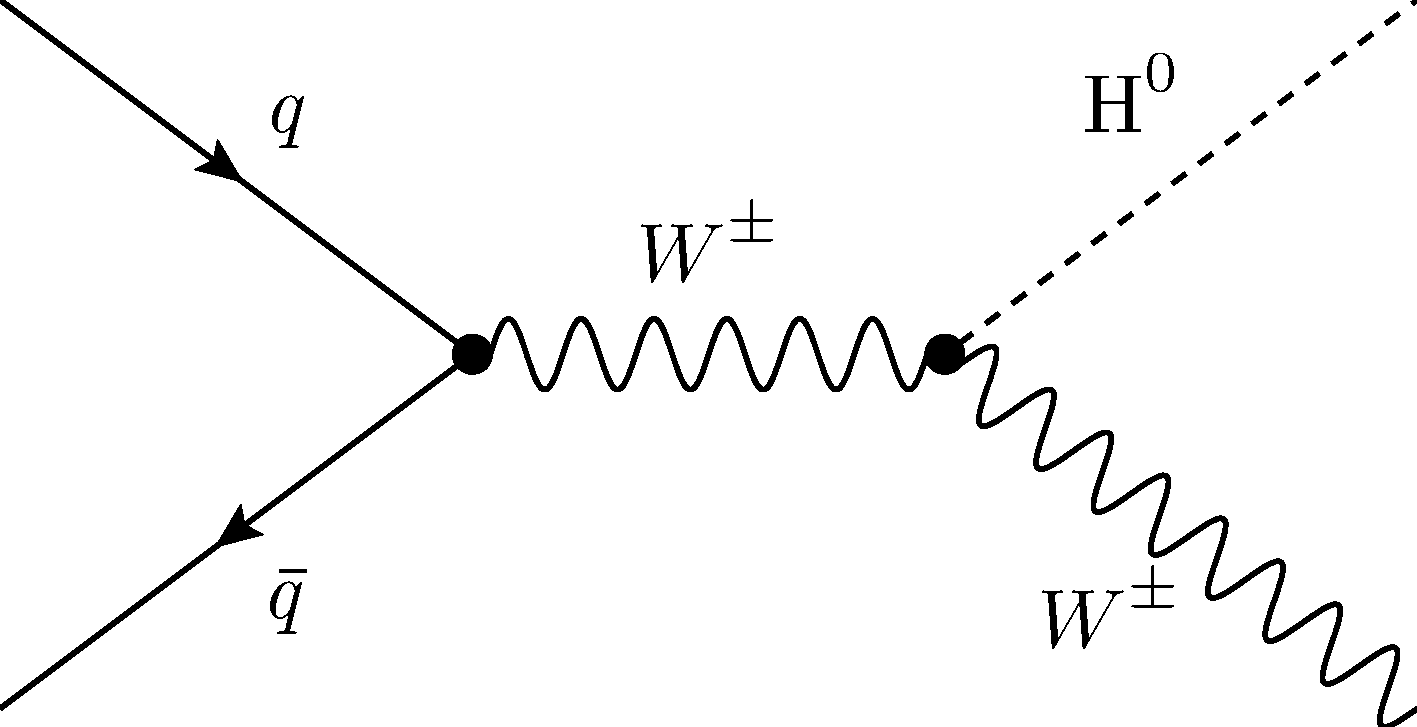
\includegraphics[width=\textwidth]{\figpath/FeynmanDiagramsPyFeyn/WH.pdf}
    \caption{Associated production with a vector boson}
    \label{fig:WH}
  \end{subfigure}
  \hspace{0.5cm}
  \begin{subfigure}[t]{0.415\textwidth}
    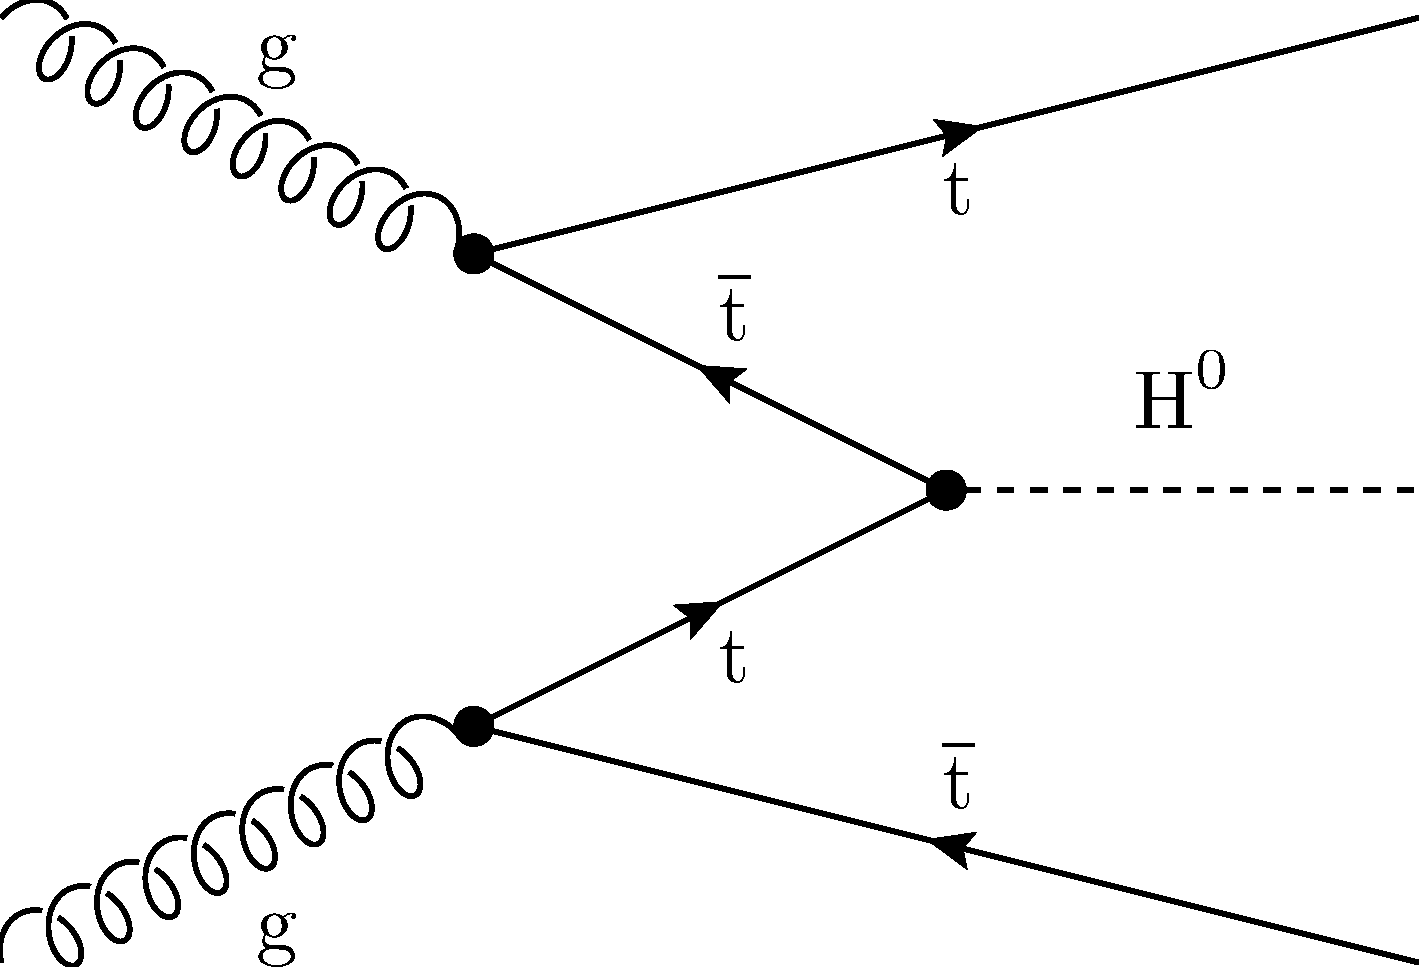
\includegraphics[width=\textwidth]{\figpath/FeynmanDiagramsPyFeyn/ttH.pdf}
    \caption{Associated production of a Higgs with a pair of t quarks}
    \label{fig:ttH}
  \end{subfigure}%
  \caption{Feynman diagrams for the four Higgs production mechanisms at the LHC.}
  \label{fig:Higgs_WW_lnujj_feynman}
\end{figure}

Just as the Higgs boson can be produced in several ways it can also decay in many ways.
Fig.~\ref{fig:Higgs_XS_and_BR} shows the Higgs decay branching ratios (BR) as well as $\sigma\times\text{BR}$ for final states containing four fermions.
It is clear from fig.~\ref{fig:Higgs_BR} that the \WW decay has one of the highest branching ratios and from fig.~\ref{fig:Higgs_XSBR_4fermion} that the \lvqq final state has the highest $\sigma\times\text{BR}$.

Given the production cross sections and branching ratios discussed above, fig.~\ref{fig:ggH_WW_lvjj} shows the dominant Feynman diagram searched for in this analysis, the gluon-gluon fusion production and semi-leptonic \W decay mode.
Nevertheless, we search for a given final state and not an exact production and decay chain, so there are several branching ratios which are useful to this analysis and are listed in table~\ref{tab:Higgs_BR}.
The $\PH\rightarrow\ZZ$ and $\PH\rightarrow\bbbar$ BR are included because they can produce a \lvqq final state given a mis-identification or mis-reconstruction issue.
The signal cross sections used in this analysis are listed in table~\ref{tab:Higgs_XS_BR} and present a couple of insights into our signal makeup.
First is that the gluon-gluon fusion process is indeed dominant with $\sim$10 times higher of a cross section than the other channels.
Additionally, the \WH channel where \Hbb is non-negligible and comparable in size to the VBF production mode, even though this is not the decay channel we are looking for.
By using some cuts to remove b-jets I will later show how to remove this signal contamination.

\begin{figure}[!hbt]
  \centering
  \begin{subfigure}[t]{0.475\textwidth}
  	\centering
  	\begin{tikzpicture}% based on https://tex.stackexchange.com/a/9561/ (Caramdir's fantastic answer to another question)
        \node (tiger) [anchor=south west, inner sep=0pt] {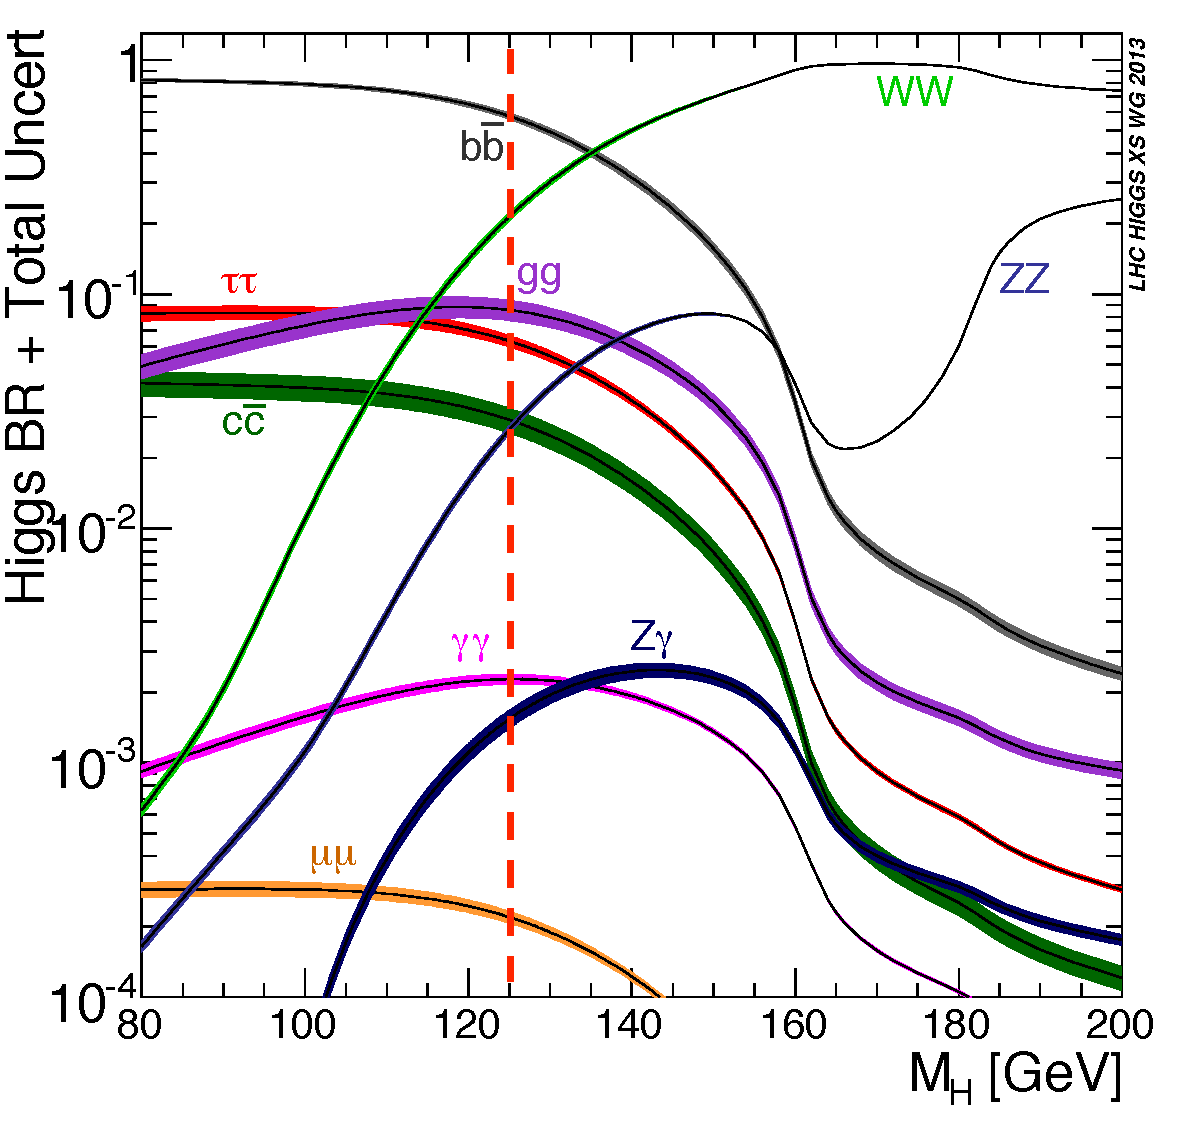
\includegraphics[width=\textwidth]{\figpath/Chapter2/Higgs_BR_LM.pdf}};
        \begin{scope}[x={(tiger.south east)},y={(tiger.north west)}]
          \foreach \i/\j in {{(0.43,0.95)/(0.43,0.12)}}
            \draw [red, very thick, dashed] \i -- \j;
        \end{scope}
    \end{tikzpicture}
    \caption{Higgs branching ratios}
    \label{fig:Higgs_BR}
  \end{subfigure}
  \begin{subfigure}[t]{0.475\textwidth}
  	\centering
    \begin{tikzpicture}% based on https://tex.stackexchange.com/a/9561/ (Caramdir's fantastic answer to another question)
        \node (tiger) [anchor=south west, inner sep=0pt] {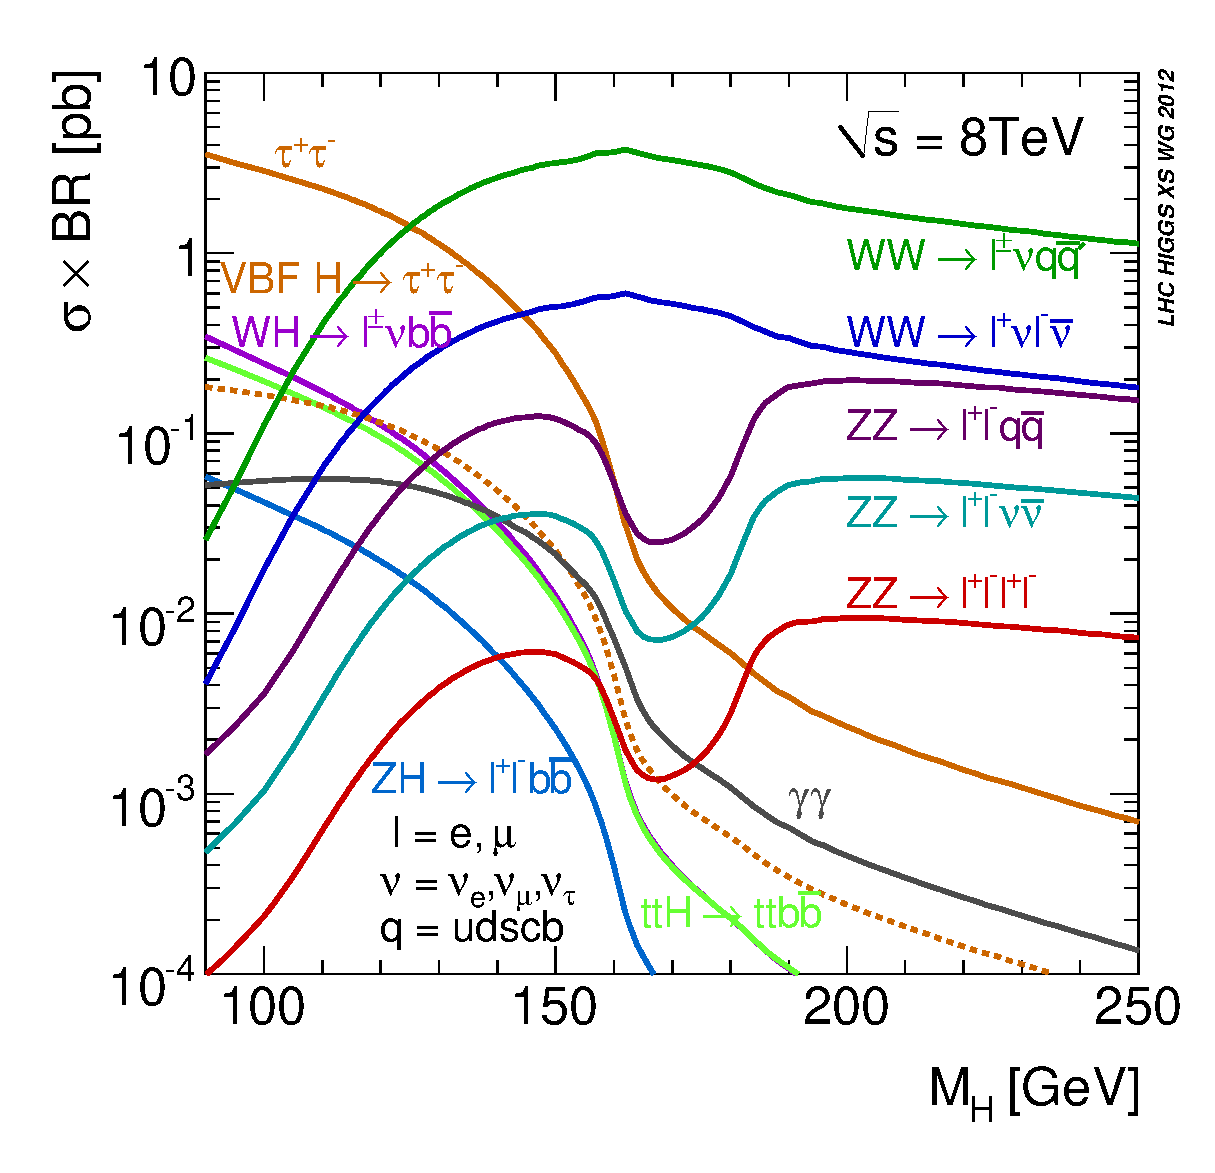
\includegraphics[width=\textwidth]{\figpath/Chapter2/XSBR_8TeV_SM_LM.eps}};
        \begin{scope}[x={(tiger.south east)},y={(tiger.north west)}]
          \foreach \i/\j in {{(0.335,0.94)/(0.335,0.15)}}
            \draw [red, very thick, dashed] \i -- \j;
        \end{scope}
    \end{tikzpicture}
    \caption{Higgs $\sigma\times\text{BR}$ for four fermion final states}
    \label{fig:Higgs_XSBR_4fermion}
  \end{subfigure}
  \caption{The dominant Higgs decay modes at the LHC. The vertical, dashed red line indicates a Higgs mass of 125\gev.}
  \label{fig:Higgs_XS_and_BR}
\end{figure}

\begin{figure}[bt]
  \centering
  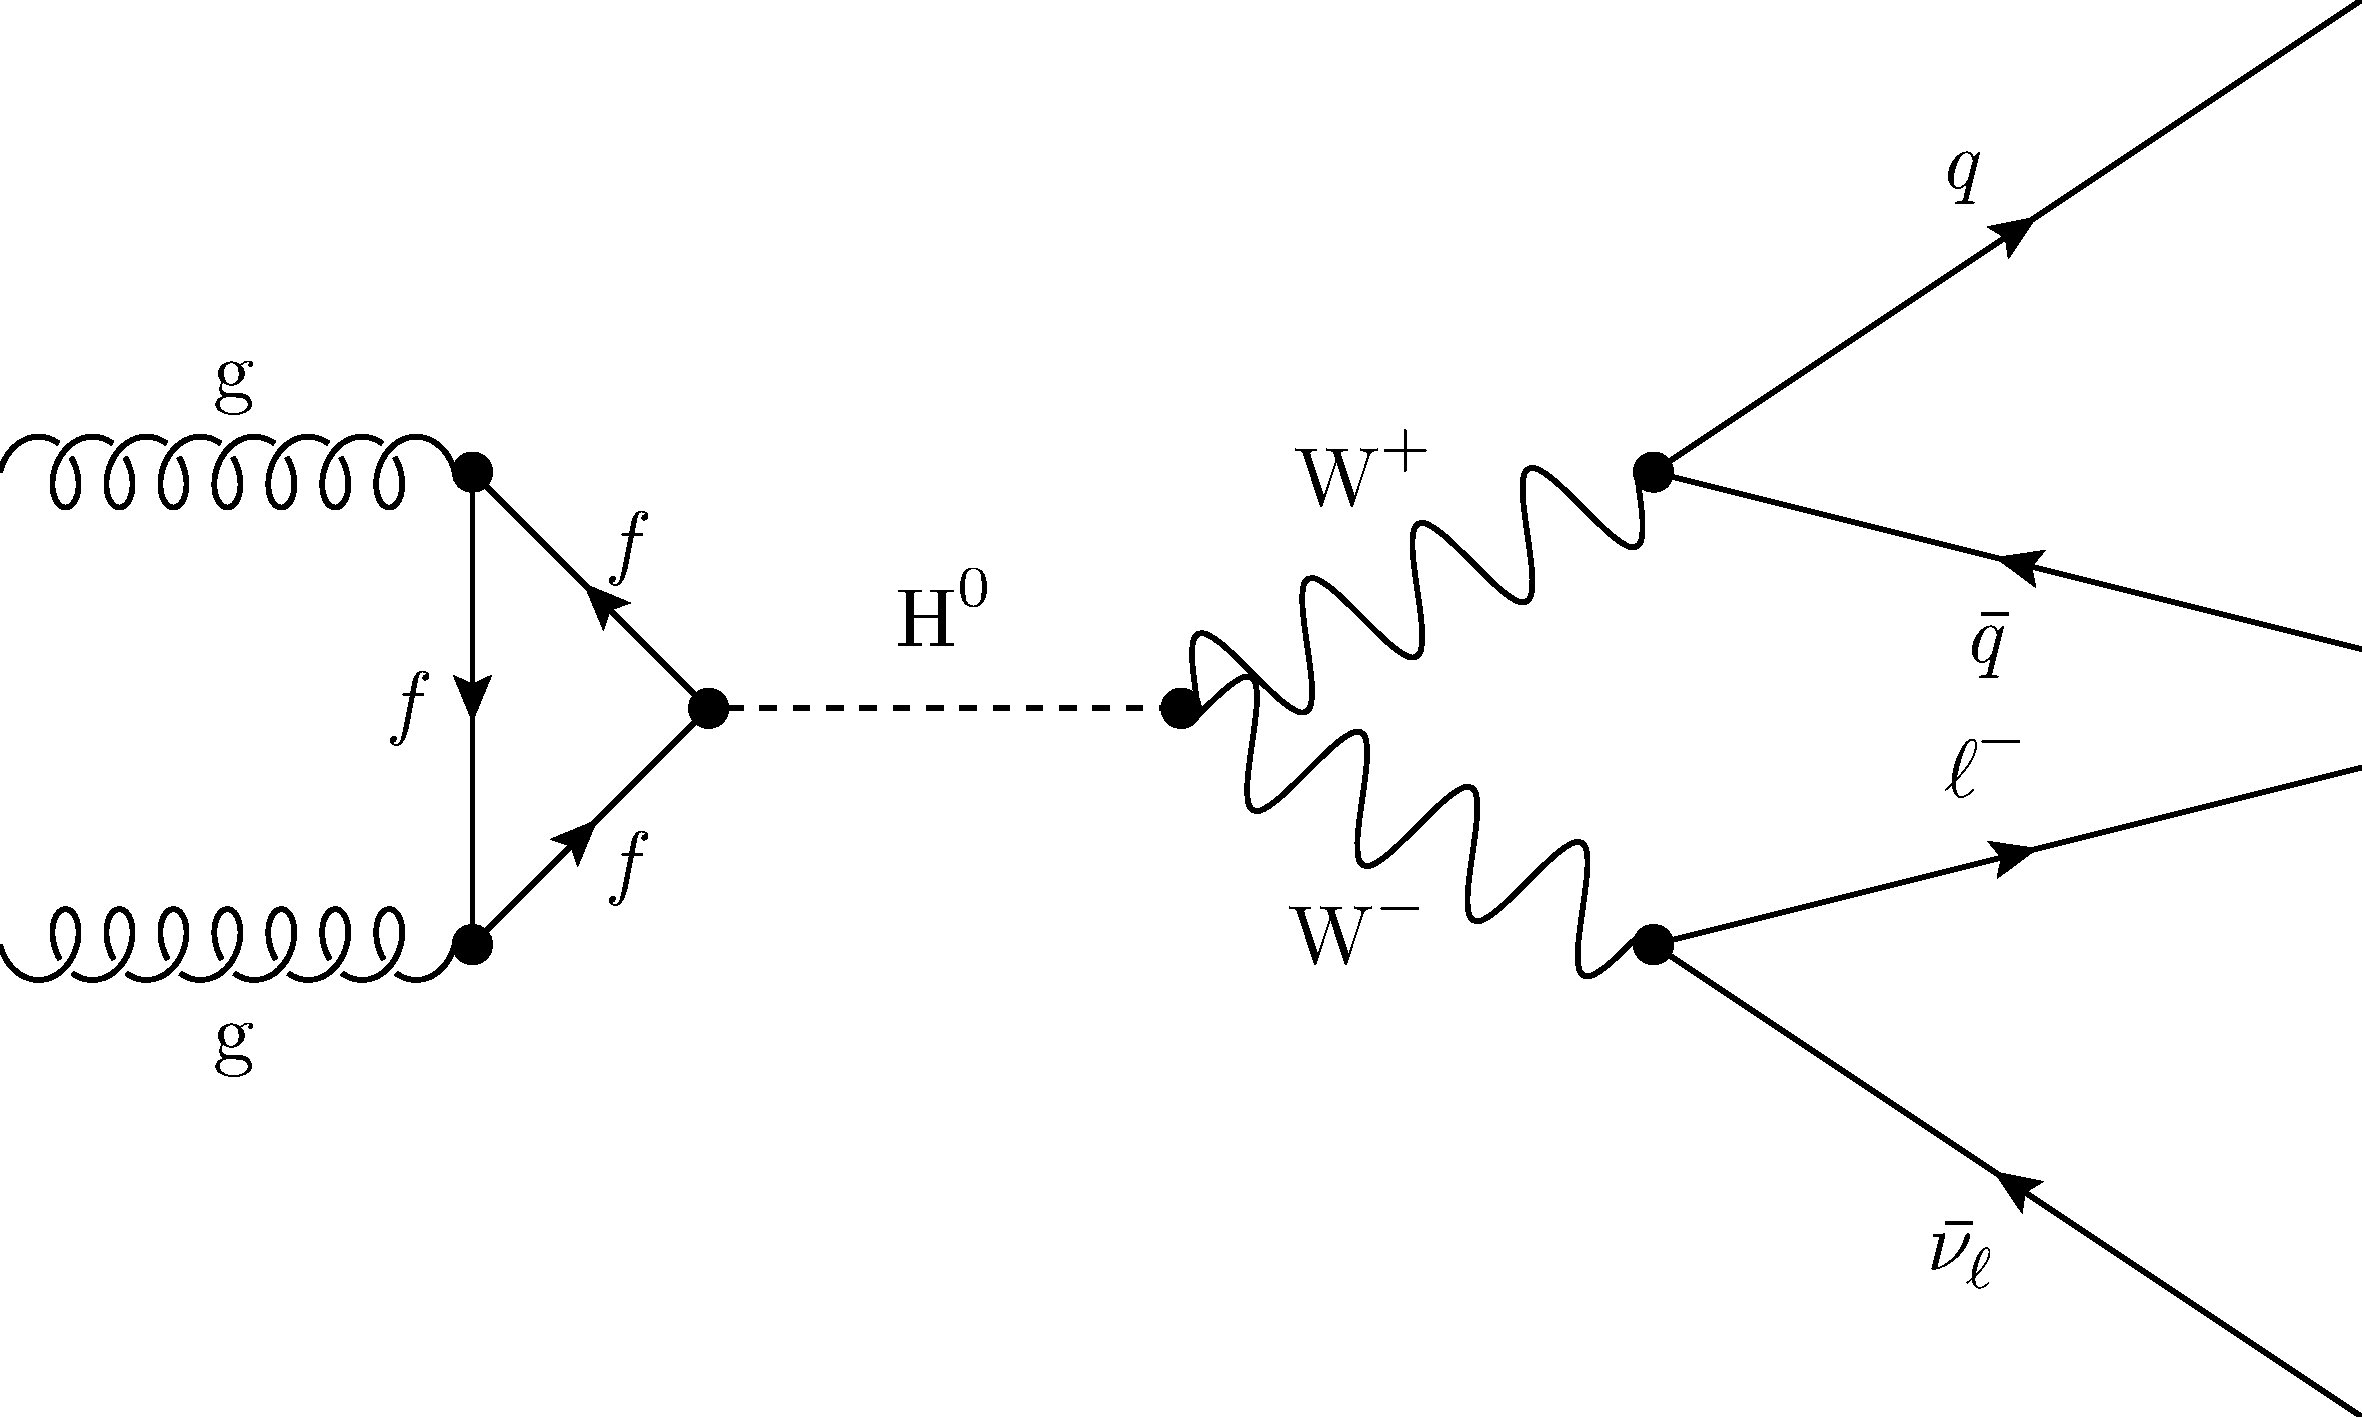
\includegraphics[width=0.95\textwidth]{\figpath/FeynmanDiagramsPyFeyn/ggH_WW_lvjj.pdf}
  \caption{Feynman diagram for the gluon-gluon fusion SM Higgs production process where the Higgs decays semi-leptonically to two quarks, one lepton, and one neutrino.}
  \label{fig:ggH_WW_lvjj}
\end{figure}

\begin{table}[htbp]
    \caption{Useful Higgs and \W branching ratios}
    \centering
    \begin{tabular}{lr}
        \hline
        Decay & BR \\
        \hline
        $\PH{\rightarrow}\WW$ & $\text{0.215}_{-\text{4.20\%}}^{+\text{4.26\%}}$ \\
        $\W{\rightarrow}l\nu$ & 0.3257 \\
        $\W{\rightarrow}\cPq\cPq$ & 0.676 \\
        $\WWlvqq$ & 0.2203 \\
        $\PH\rightarrow\ZZ$ & $\text{0.0246}_{-\text{4.21\%}}^{+\text{4.28\%}}$ \\
        $\PH\rightarrow\bbbar$ & $\text{0.577}_{-\text{3.27\%}}^{+\text{3.21\%}}$ \\
        \hline
    \end{tabular}
    \label{tab:Higgs_BR}
\end{table}

\begin{table}[htbp]
    \caption{A table of $\sigma\times\text{BR}$ for the \lvqq final state resulting from any Higgs production mode and several decay channels.}
    \centering
    \begin{tabular}{lr}
        \hline
        Channel & $\sigma\times\text{BR}$ \\
        \hline
        \ggH, where \HWWlvqq & 1.823\pbinv \\
        \qqH, where \HWWlvqq & 0.1493\pbinv \\
        \WH, where \HWW & 0.1515\pbinv \\
        \ZH, where \HWW & 0.08929\pbinv \\
        \ttH, where \HWW & 0.0278\pbinv \\
        \WH, where \Hbblvqq & 0.1324\pbinv \\
        \ttH, where \Hbblvqq & 0.0746\pbinv \\
        \WH, where \HZZ & 0.01860\pbinv \\
        \ZH, where \HZZ & 0.01096\pbinv \\
        \ttH, where \HZZ & 0.00341\pbinv \\
        \hline
    \end{tabular}
    \label{tab:Higgs_XS_BR}
\end{table}

In addition to the true signal events, volunteer signal events (i.e. \Hbb), this analysis must content with several other standard model processes which can produce a \lvqq final state.
These background events can even have rates several orders of magnitude higher than that of our signal.
There are two varieties of backgrounds which will be encountered, reducible and irreducible.
The irreducible backgrounds, like the SM \WW process, will exactly produce the \lvqq final state.
On the other hand, reducible backgrounds produce slightly different final states, but may still enter the signal region for a variety of reasons.
An example of a reducible background is the \ttbar process, which will have extra (b-)jets that may be removed through additional cuts.

\begin{figure}[!hbt]
  \centering
  \begin{subfigure}[t]{0.46\textwidth}
    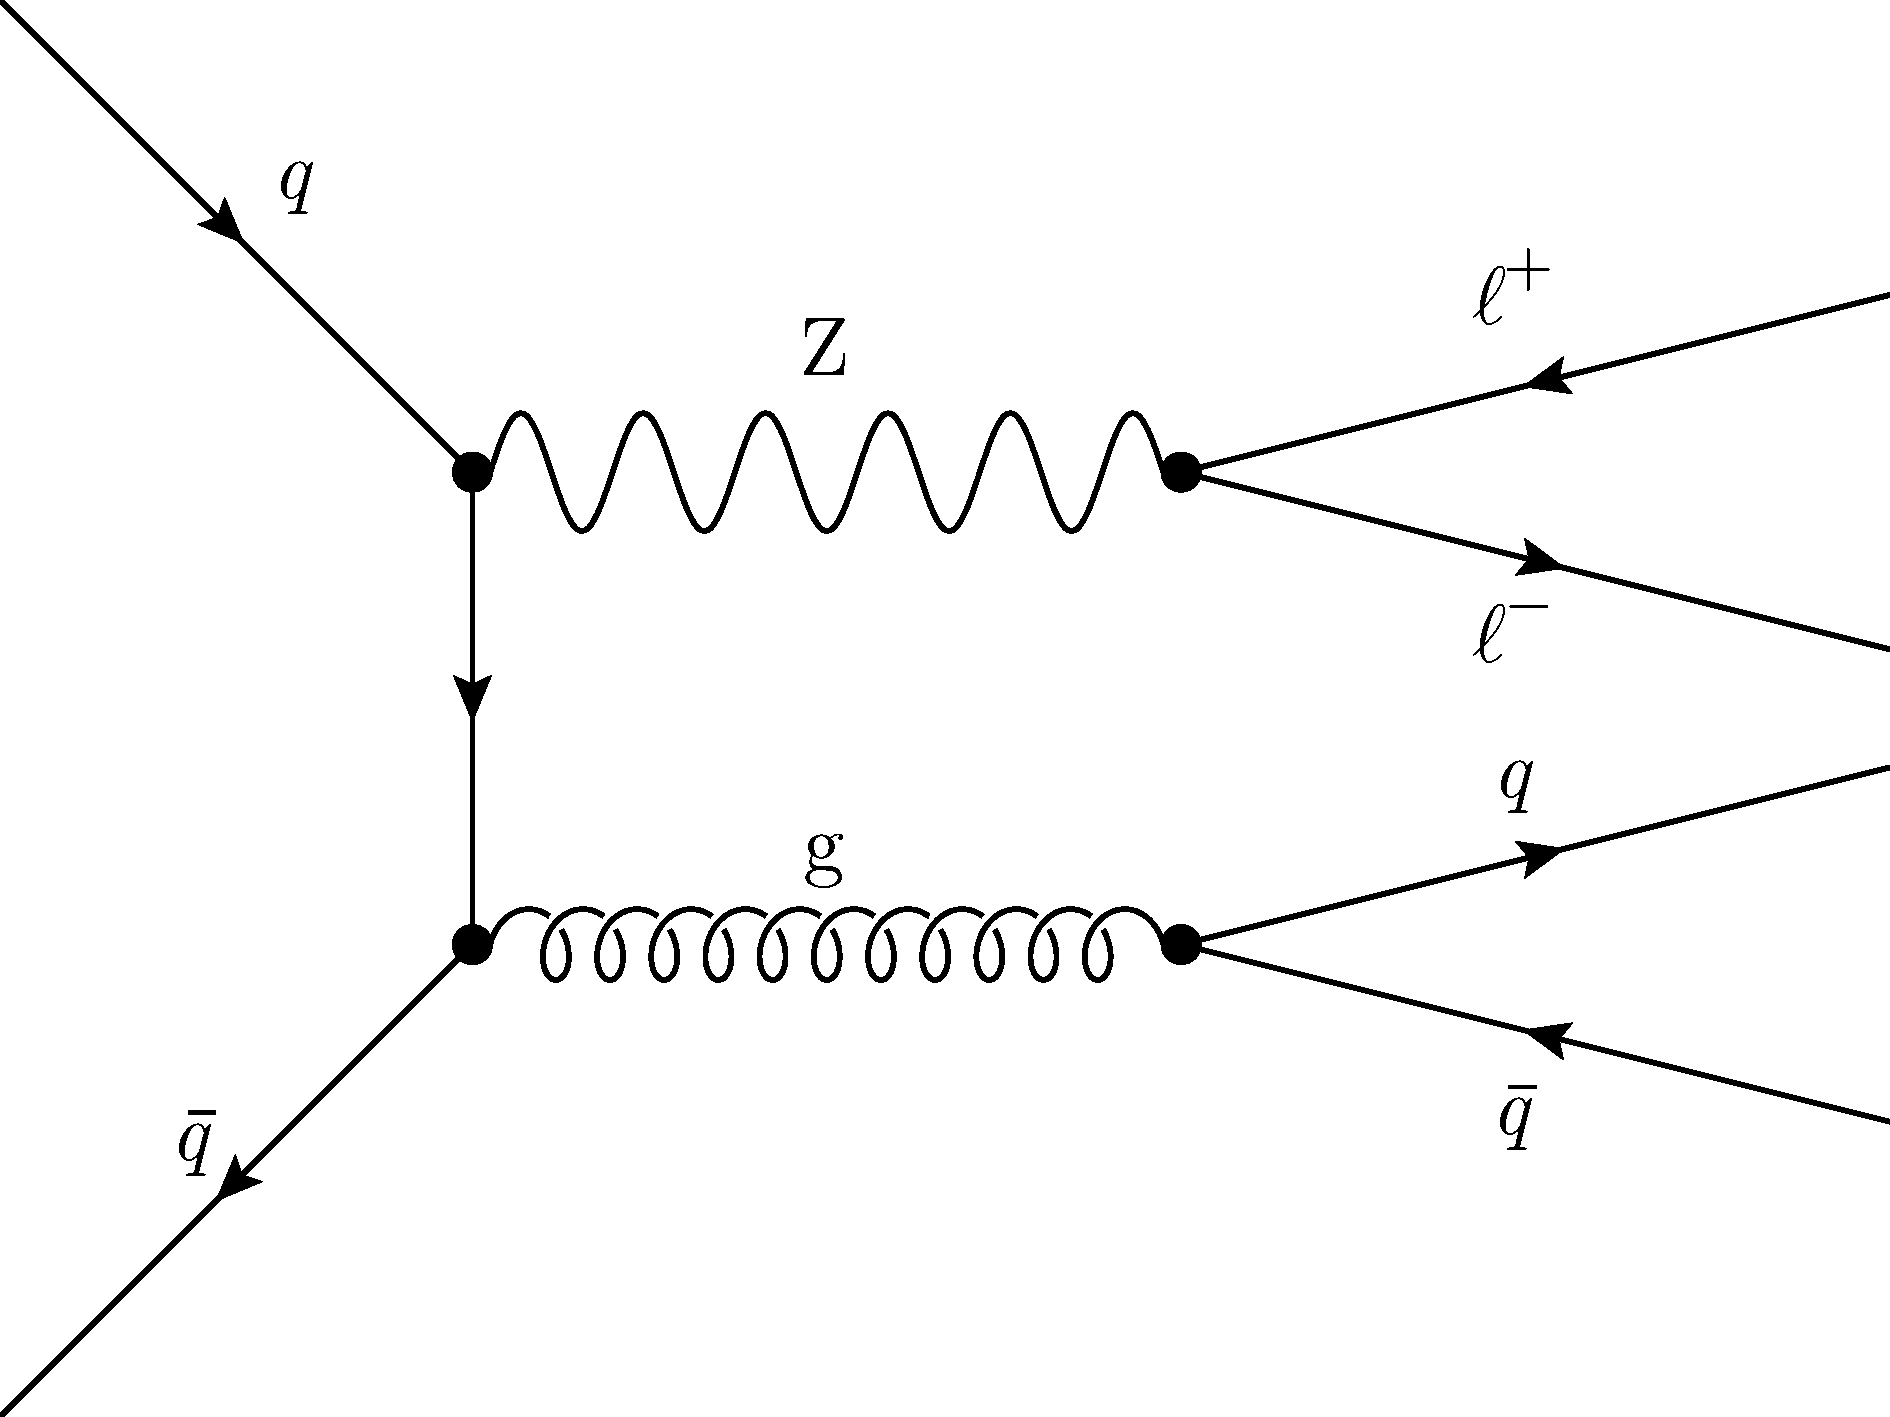
\includegraphics[width=\textwidth]{\figpath/FeynmanDiagramsPyFeyn/ZJets.pdf}
  	\caption{$Z^{0}$ production in association with jets}
    \label{fig:ZJets_lvjj}
  \end{subfigure}
  \hspace{0.015\textwidth}
  \begin{subfigure}[t]{0.46\textwidth}
    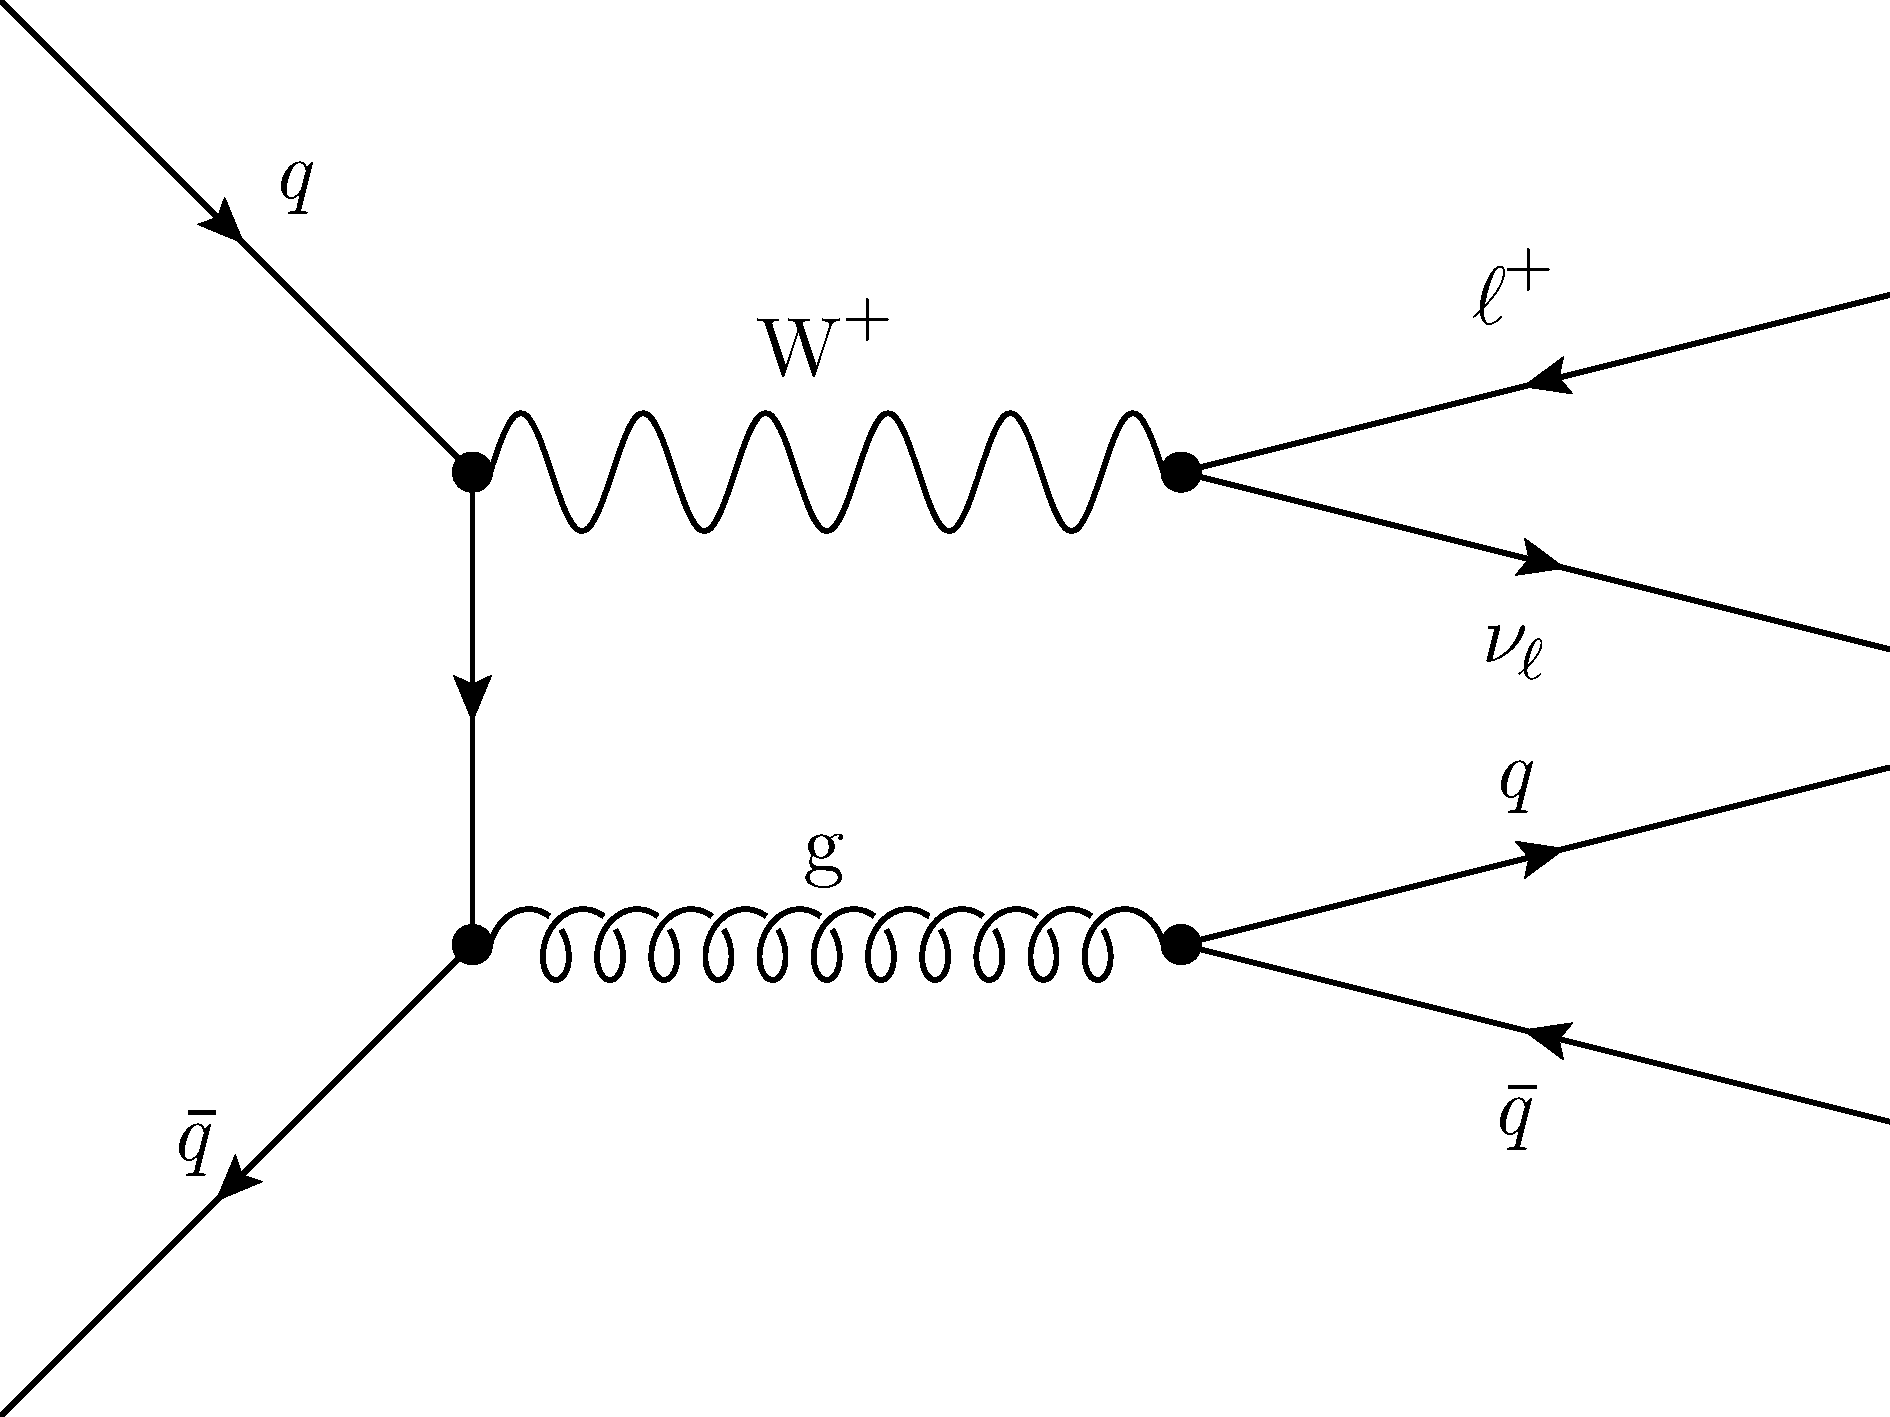
\includegraphics[width=\textwidth]{\figpath/FeynmanDiagramsPyFeyn/WJets.pdf}
    \caption{$W^{+}$ production in association with jets}
    \label{fig:WJets_lvjj}
  \end{subfigure}
  \caption{Example Feynman diagrams for the standard model $\text{V}+\text{jets}$ process decaying to the $\ell\nu{jj}$ final state.}
  \label{fig:SingleBosonBackground}
\end{figure}
\begin{figure}[!hbt]
  \centering
  \begin{subfigure}[t]{0.3\textwidth}
    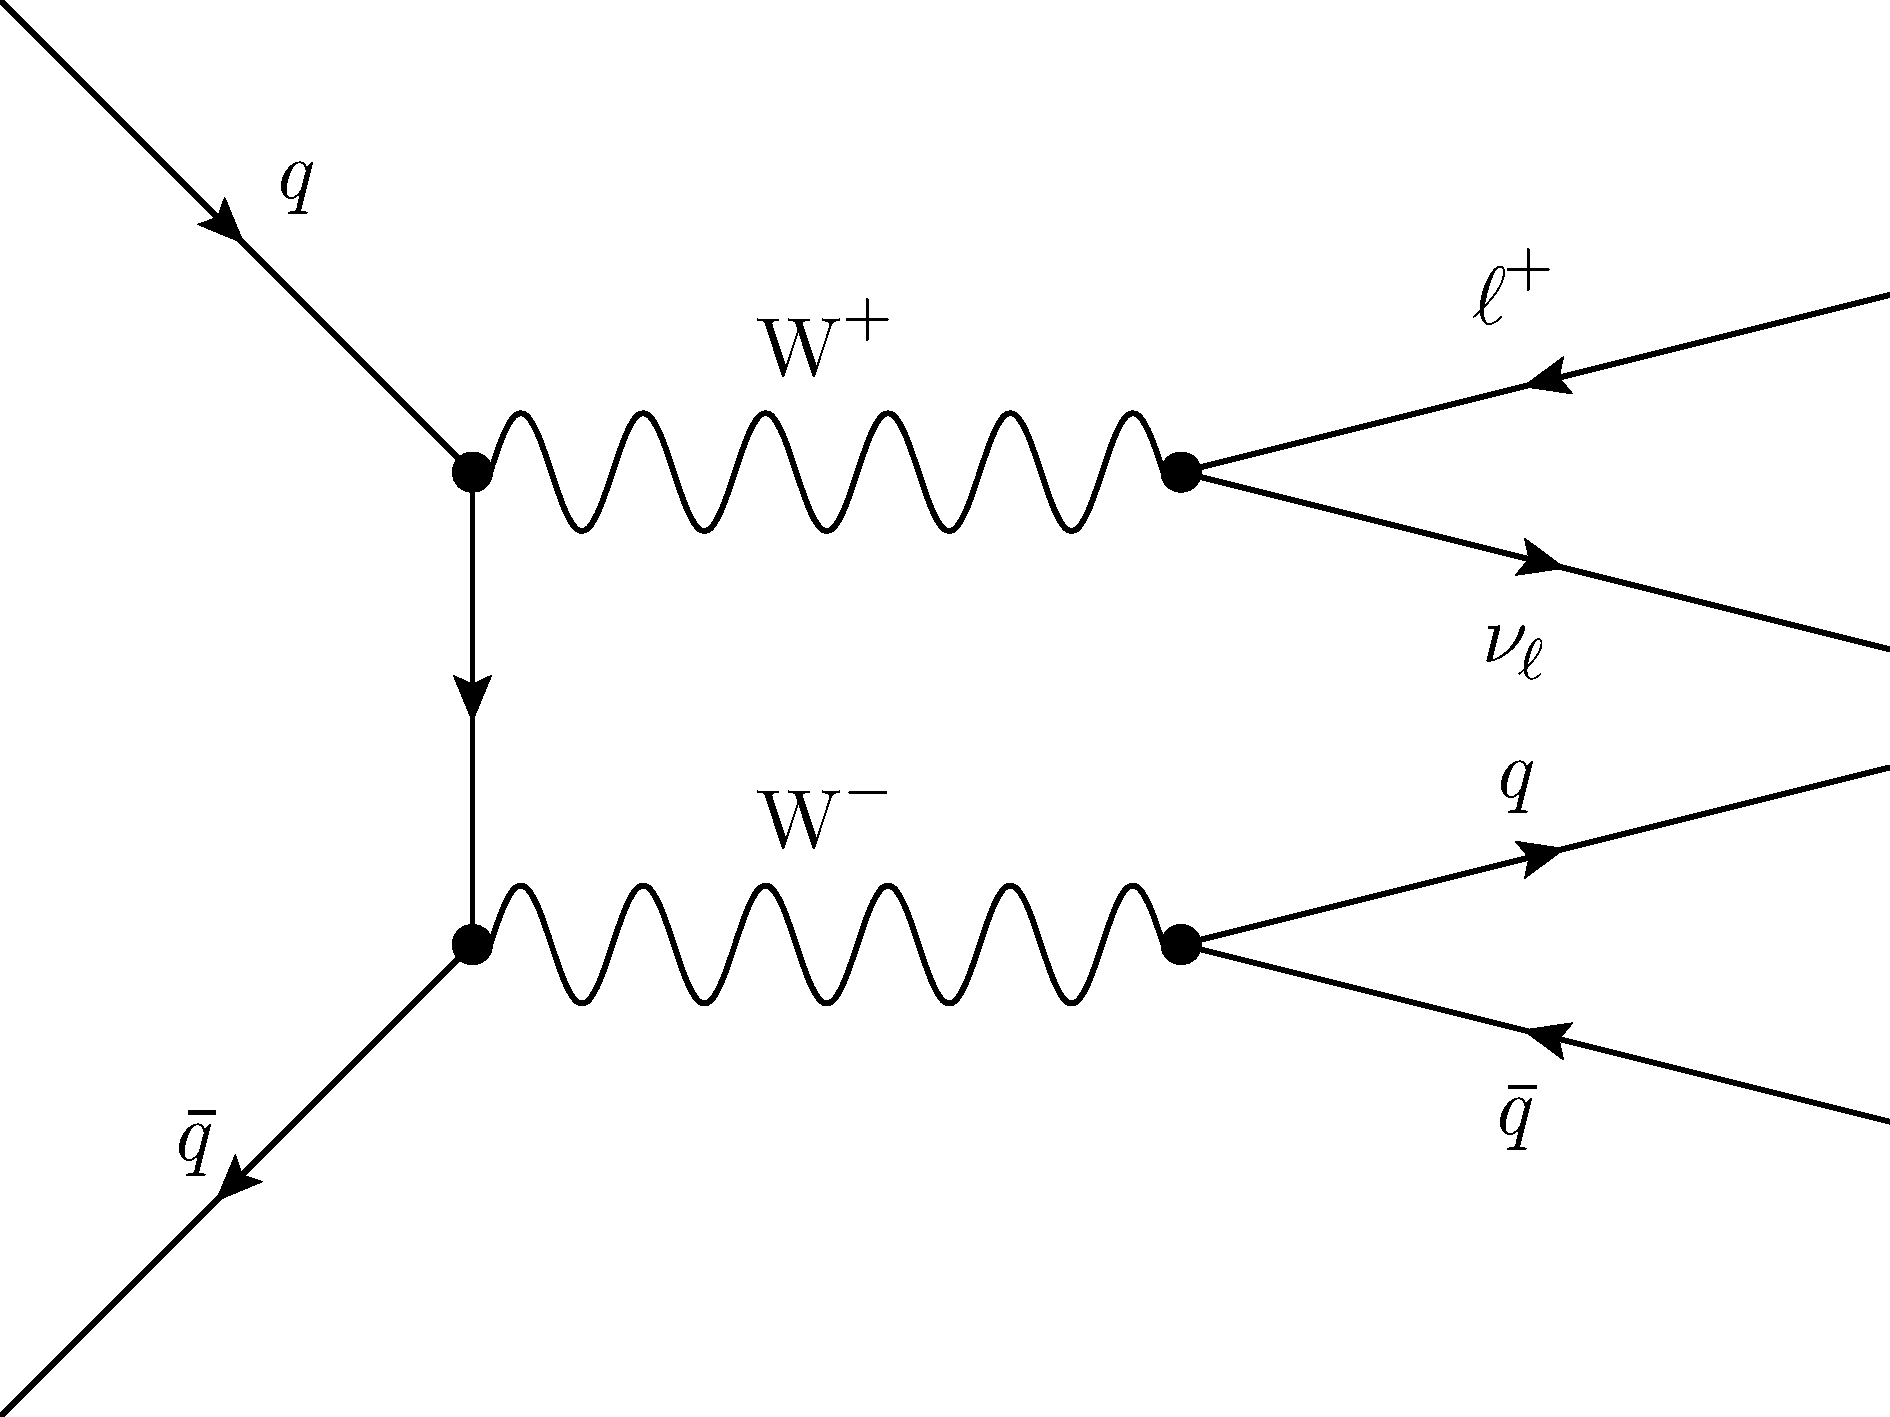
\includegraphics[width=\textwidth]{\figpath/FeynmanDiagramsPyFeyn/WW.pdf}
    \caption{$W^{+}W^{-}$ pair production}
    \label{fig:WW}
  \end{subfigure}
  \hspace{0.015\textwidth}
  \begin{subfigure}[t]{0.3\textwidth}
    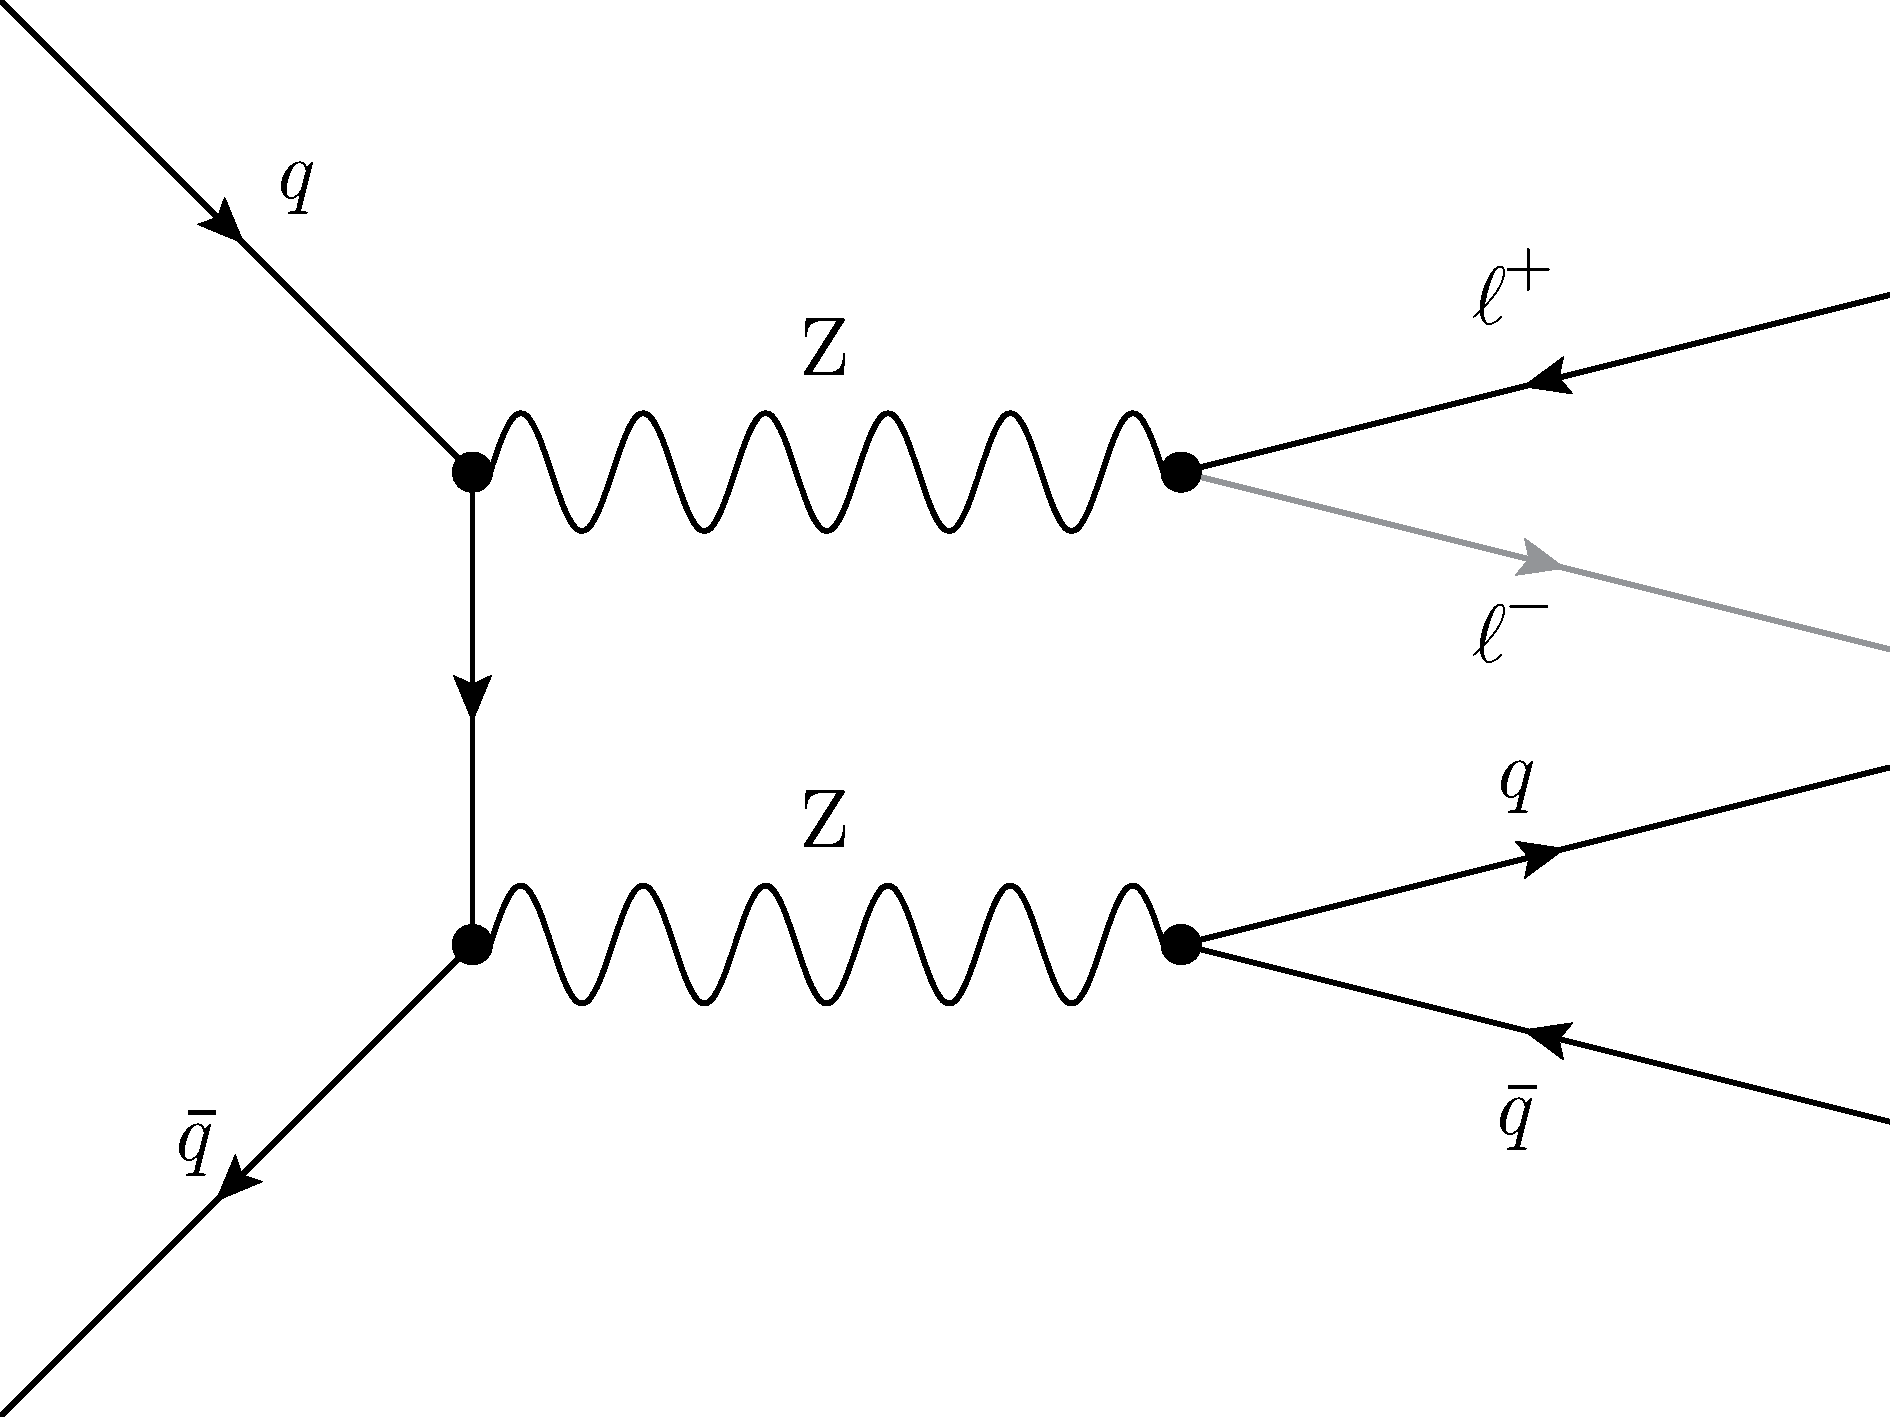
\includegraphics[width=\textwidth]{\figpath/FeynmanDiagramsPyFeyn/ZZ.pdf}
    \caption{Z boson pair production}
    \label{fig:ZZ}
  \end{subfigure}
  \hspace{0.015\textwidth}
  \begin{subfigure}[t]{0.3\textwidth}
    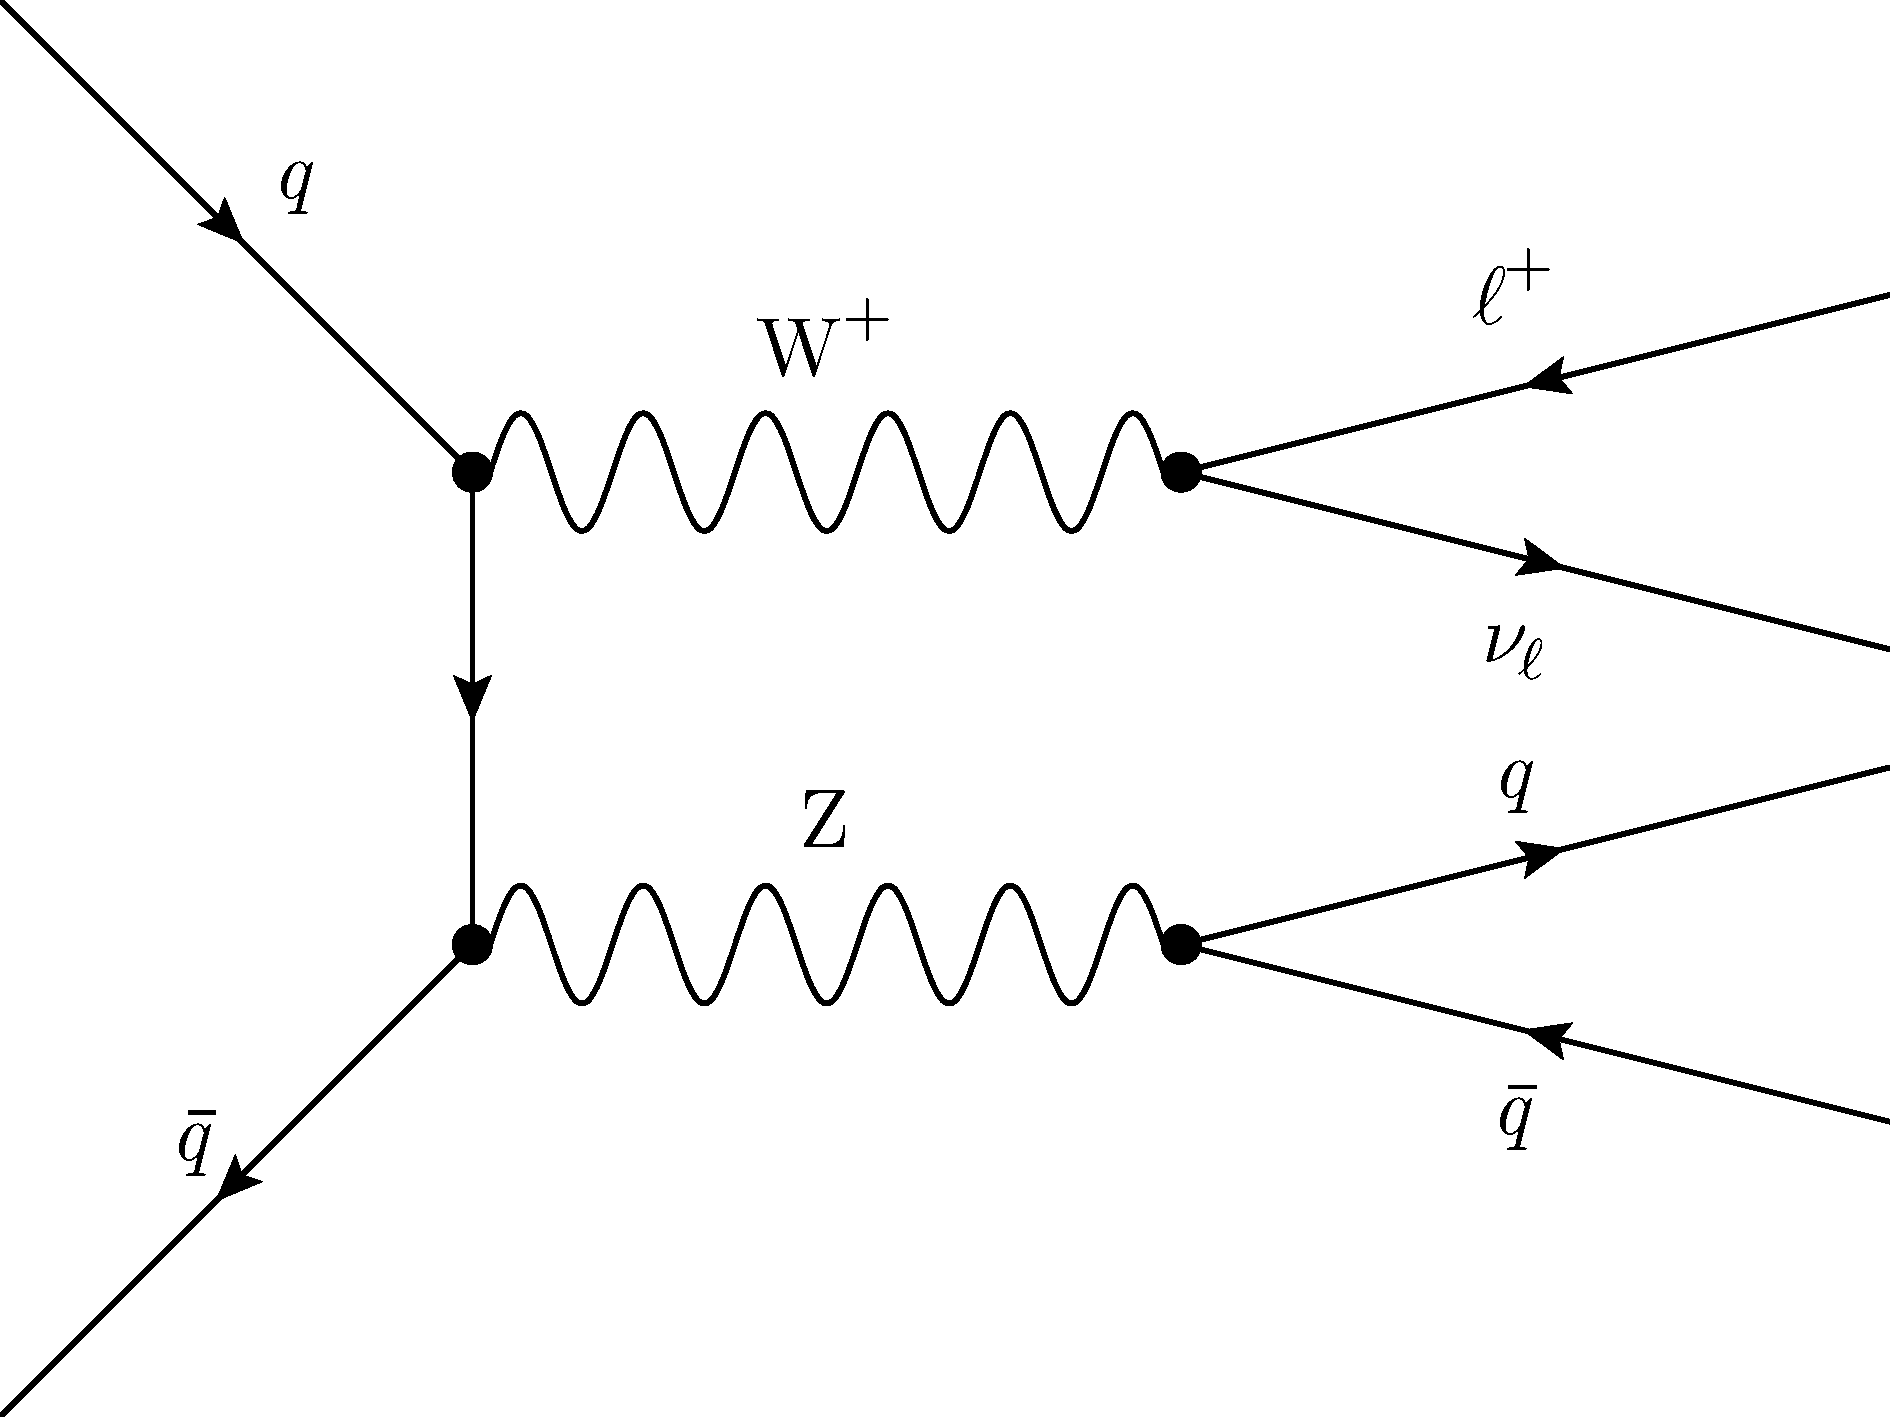
\includegraphics[width=\textwidth]{\figpath/FeynmanDiagramsPyFeyn/WZ.pdf}
    \caption{Production of a $W^{+}$ and $Z$ boson}
    \label{fig:WZ}
  \end{subfigure}
  \caption{Example Feynman diagrams for the standard model diboson processes decaying to the $\ell\nu{jj}$ final state.}
  \label{fig:DibosonBackground}
\end{figure}
\begin{figure}[!hbt]
  \centering
  \begin{subfigure}[t]{0.46\textwidth}
    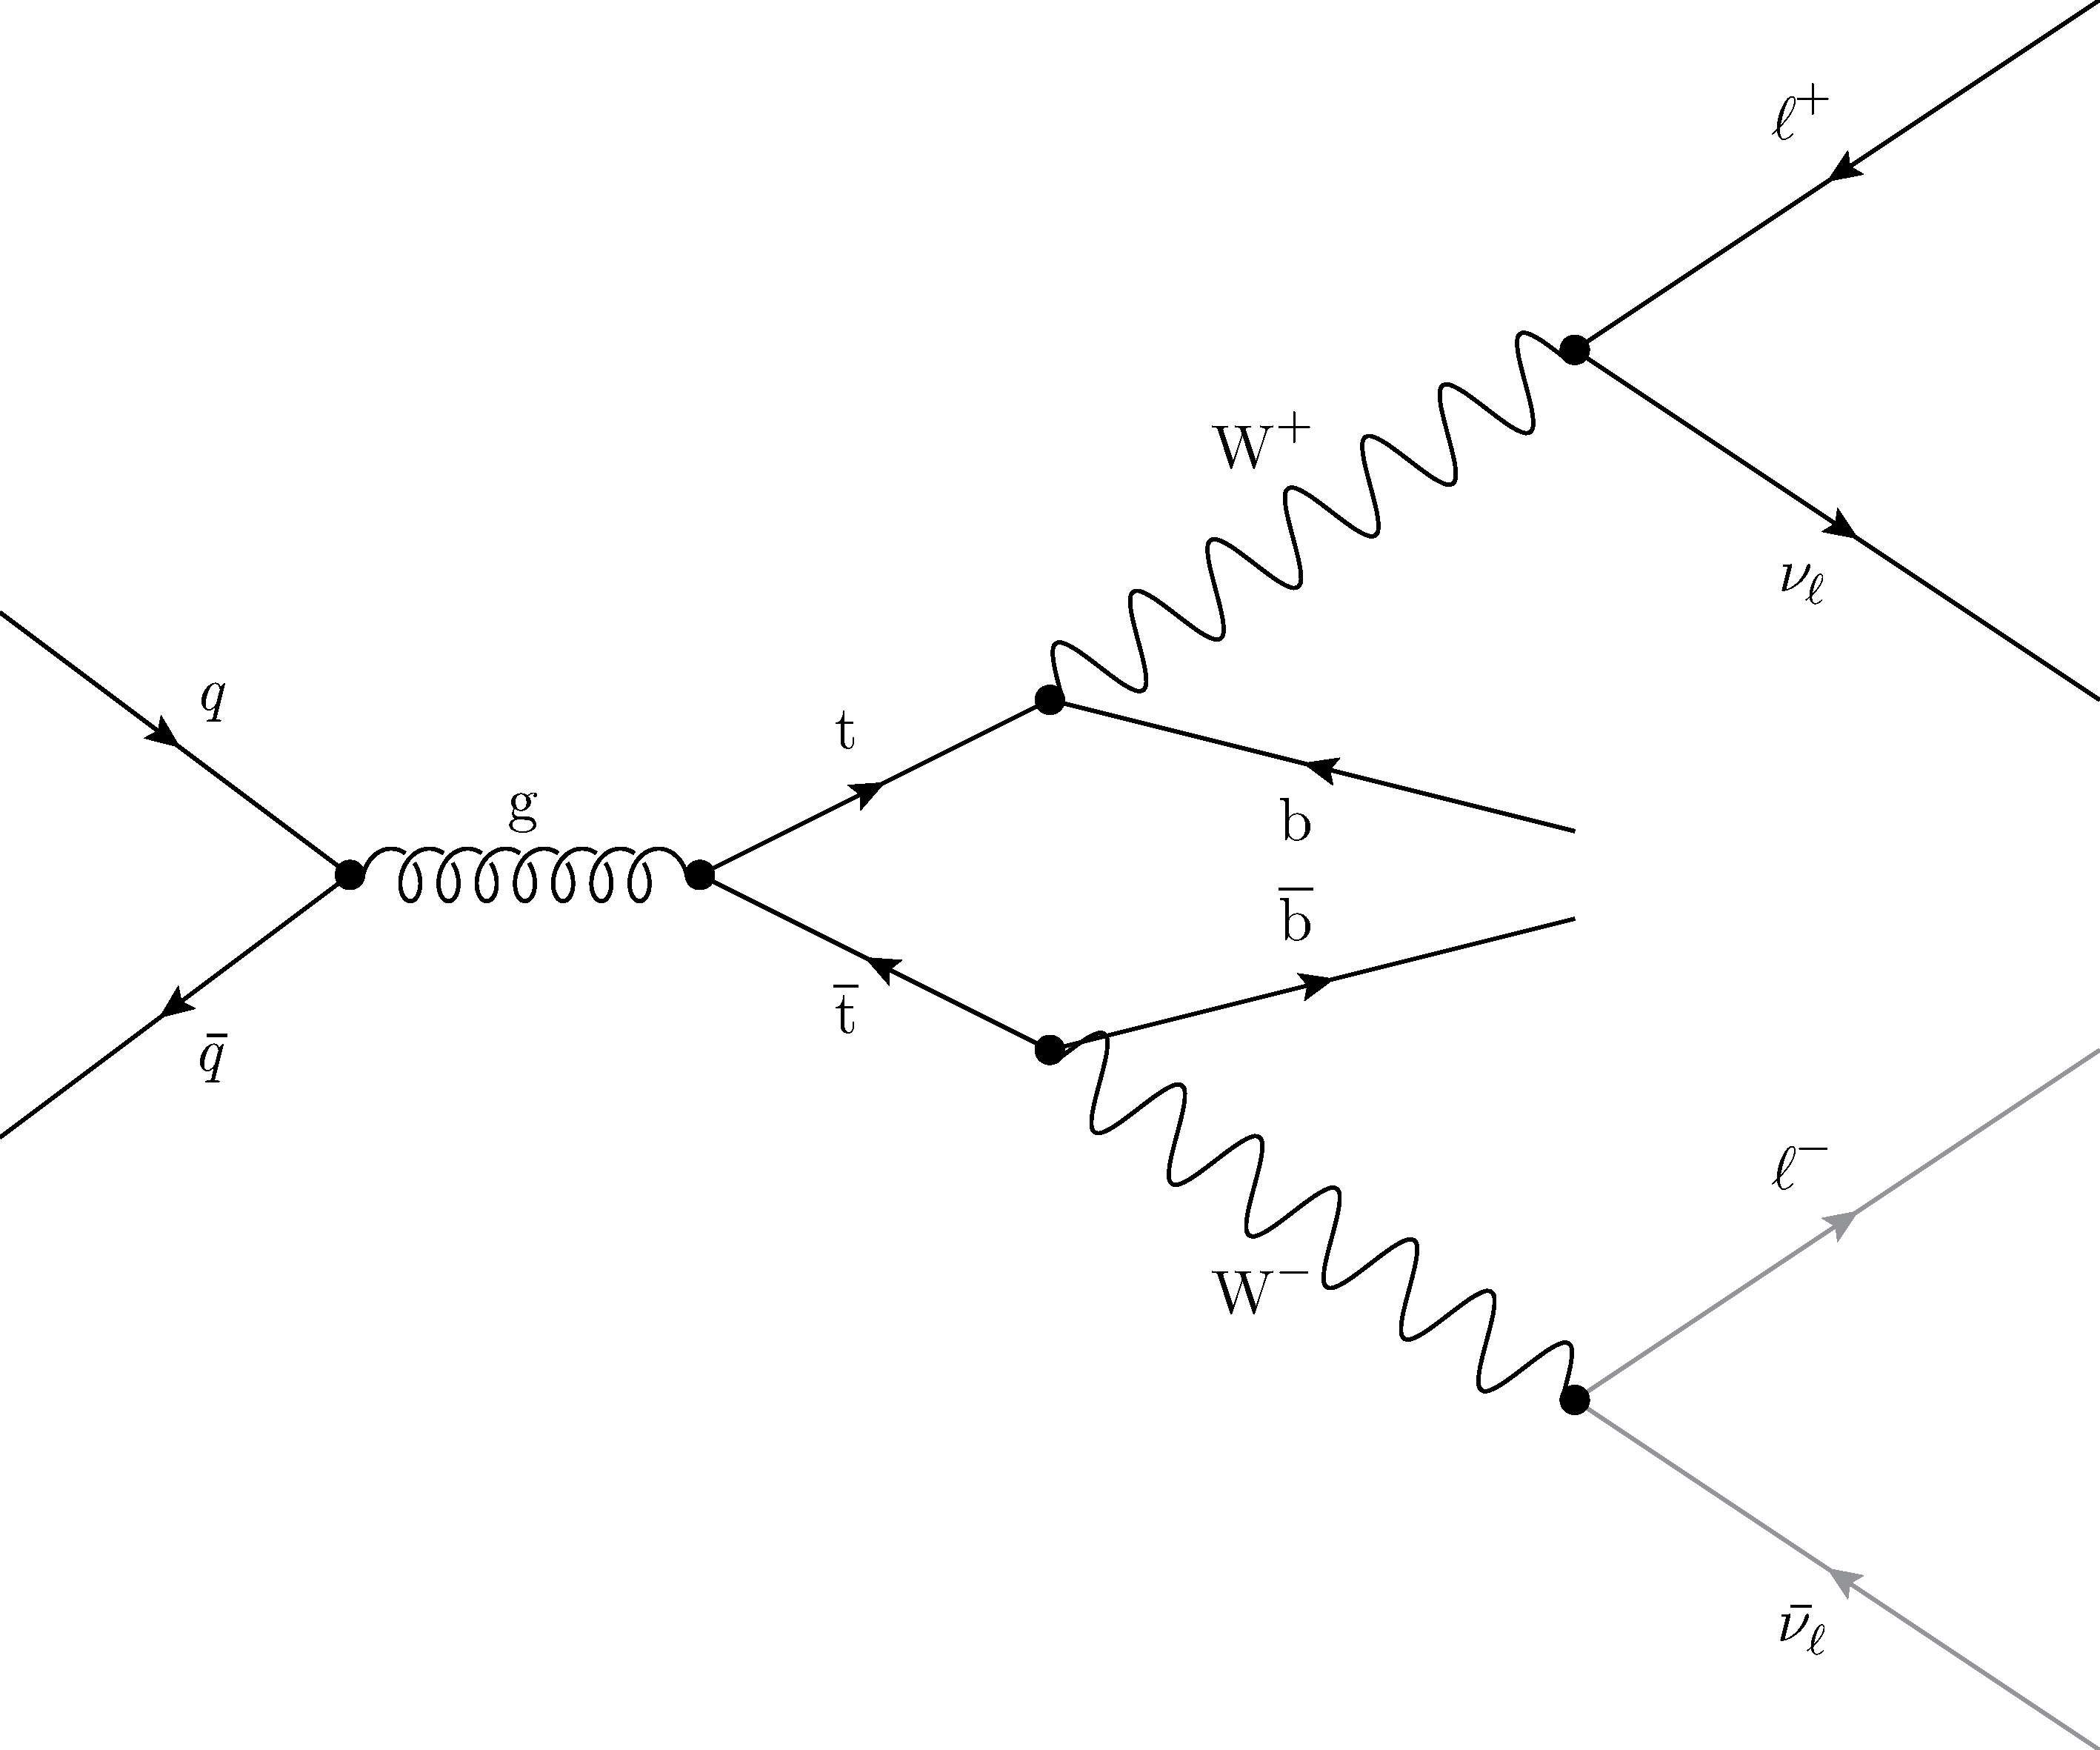
\includegraphics[width=\textwidth]{\figpath/FeynmanDiagramsPyFeyn/TTbar2.pdf}
    \caption{}
    \label{fig:TTbar_lvlvbb}
  \end{subfigure}
  \hspace{0.015\textwidth}
  \begin{subfigure}[t]{0.46\textwidth}
    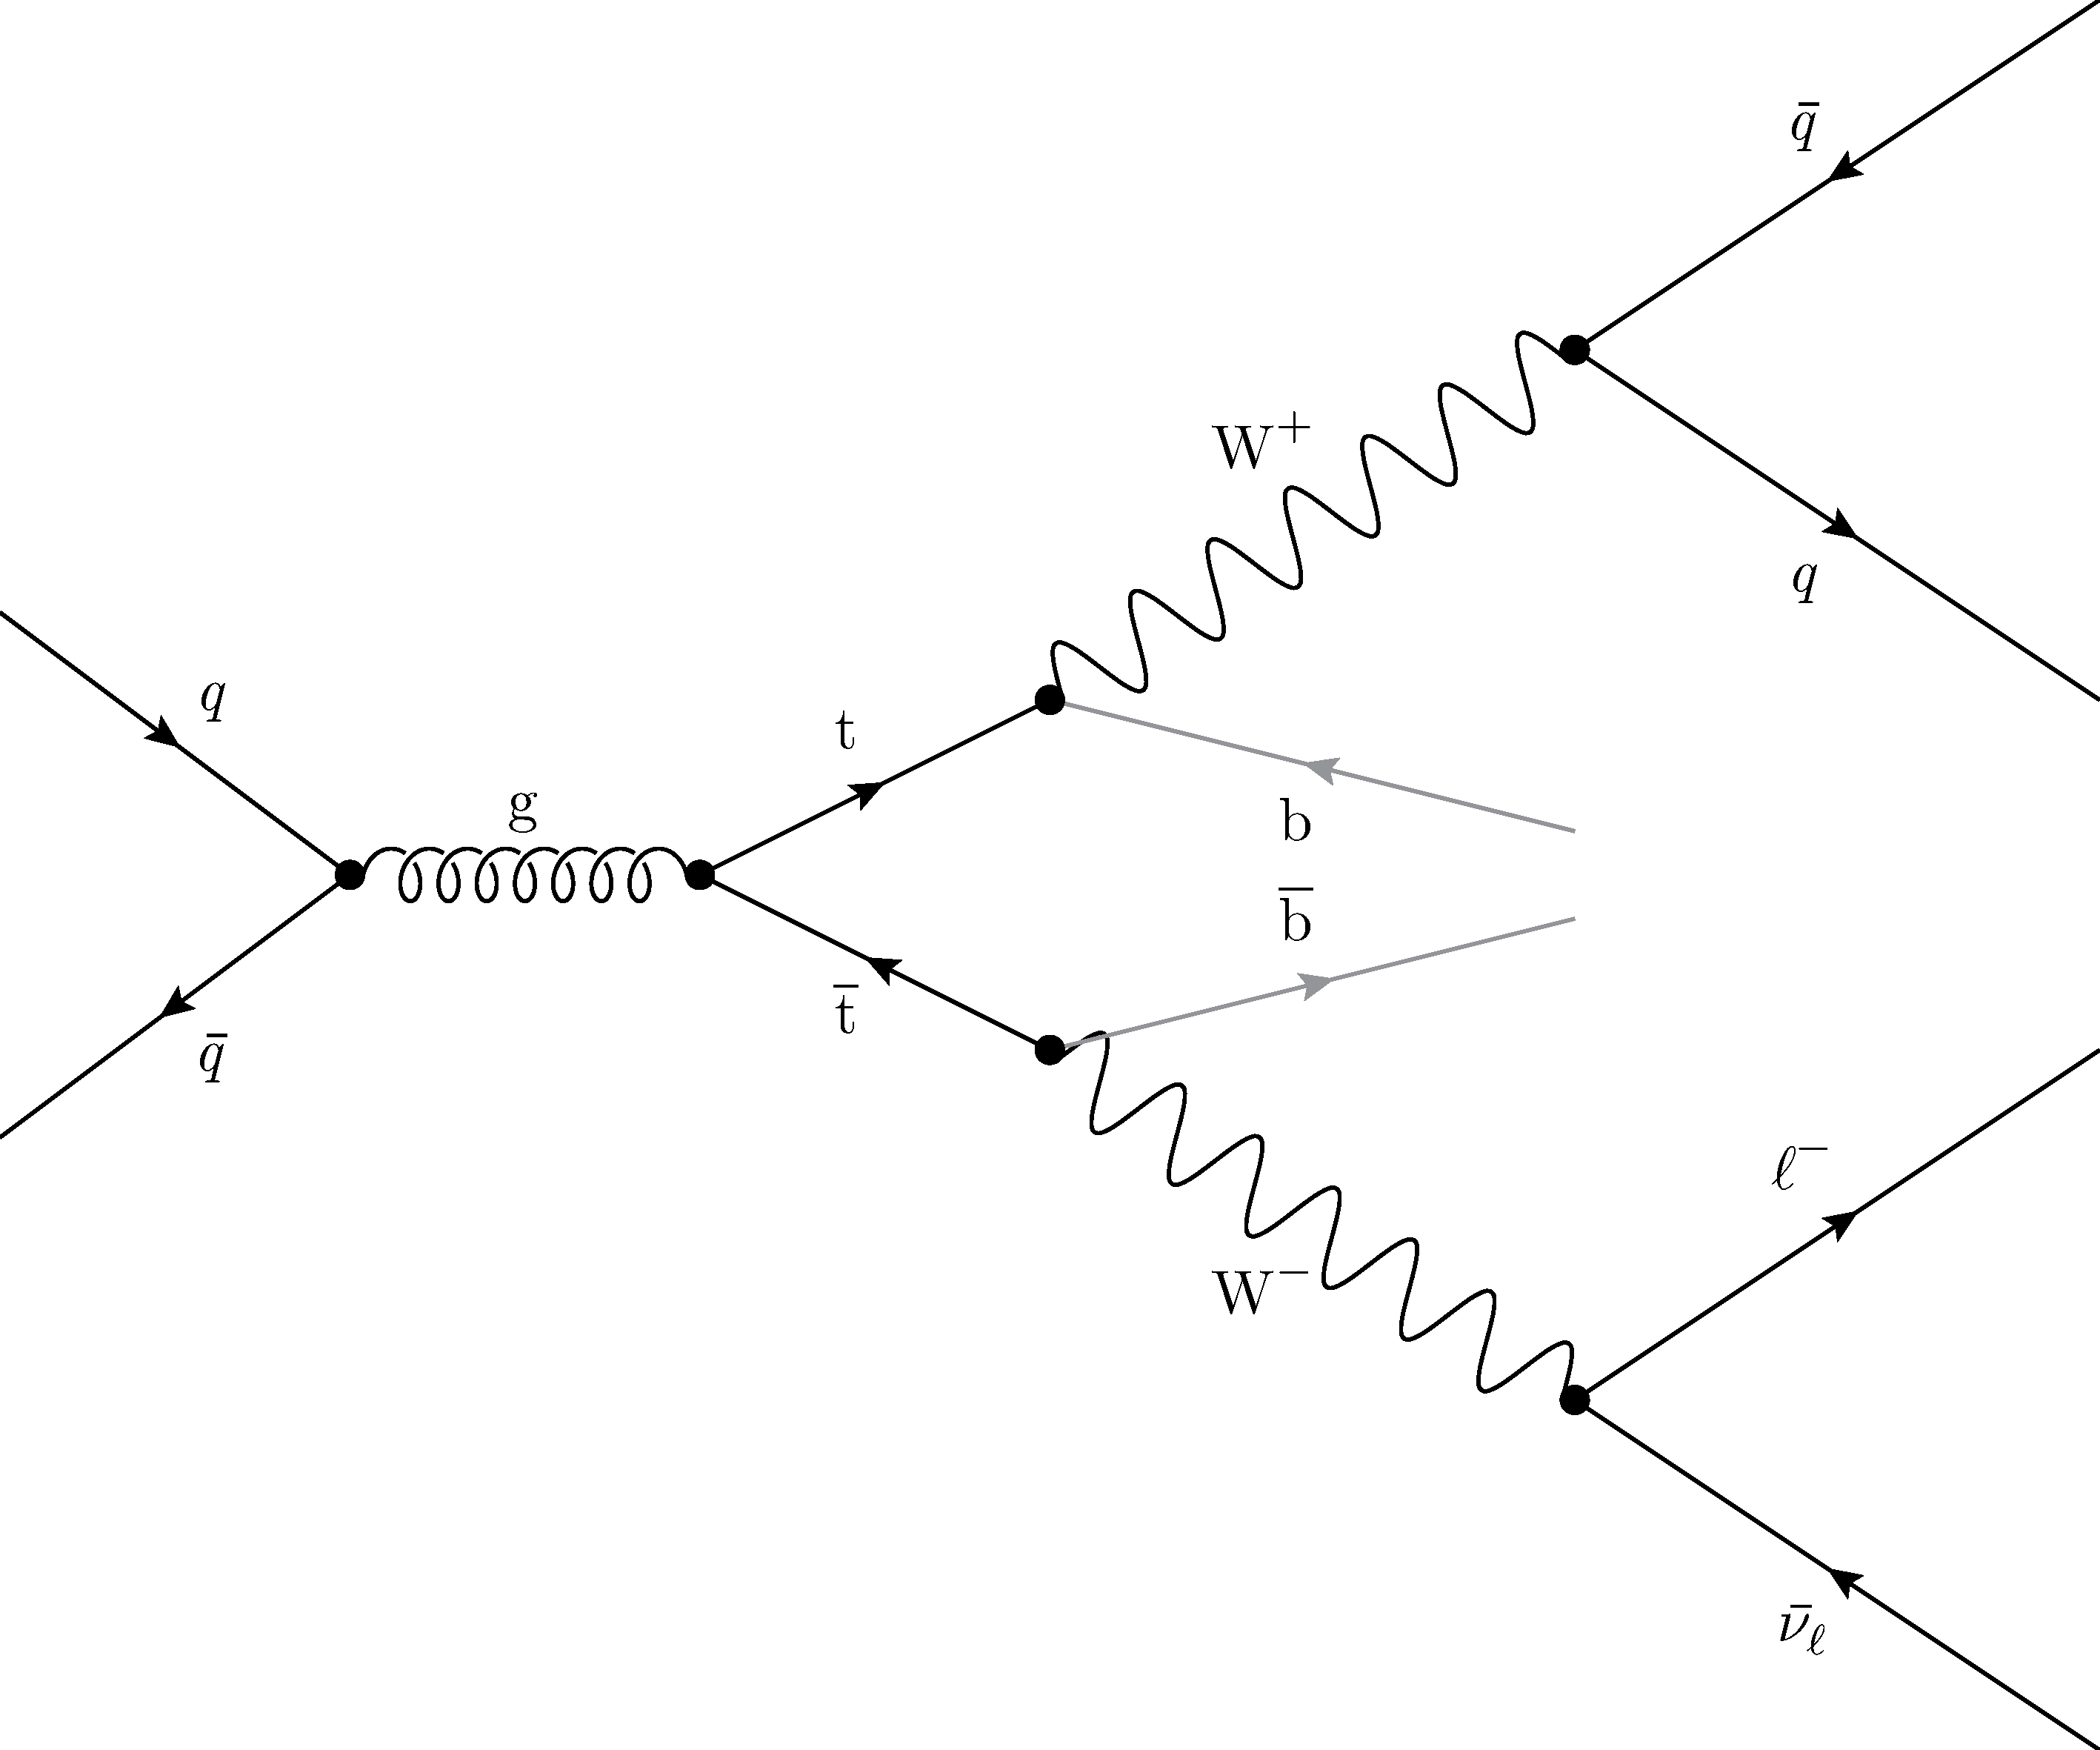
\includegraphics[width=\textwidth]{\figpath/FeynmanDiagramsPyFeyn/TTbar.pdf}
    \caption{}
    \label{fig:TTbar_lvjjbb}
  \end{subfigure}
  \caption{Two possible \ttbar Feynman diagrams which could have final states similar to the Higgs signal. Lines in gray are either mis-reconstructed or missing.}
  \label{fig:TTbarBackground}
\end{figure}
\begin{figure}[!hbt]
  \centering
  \begin{subfigure}[t]{0.3\textwidth}
    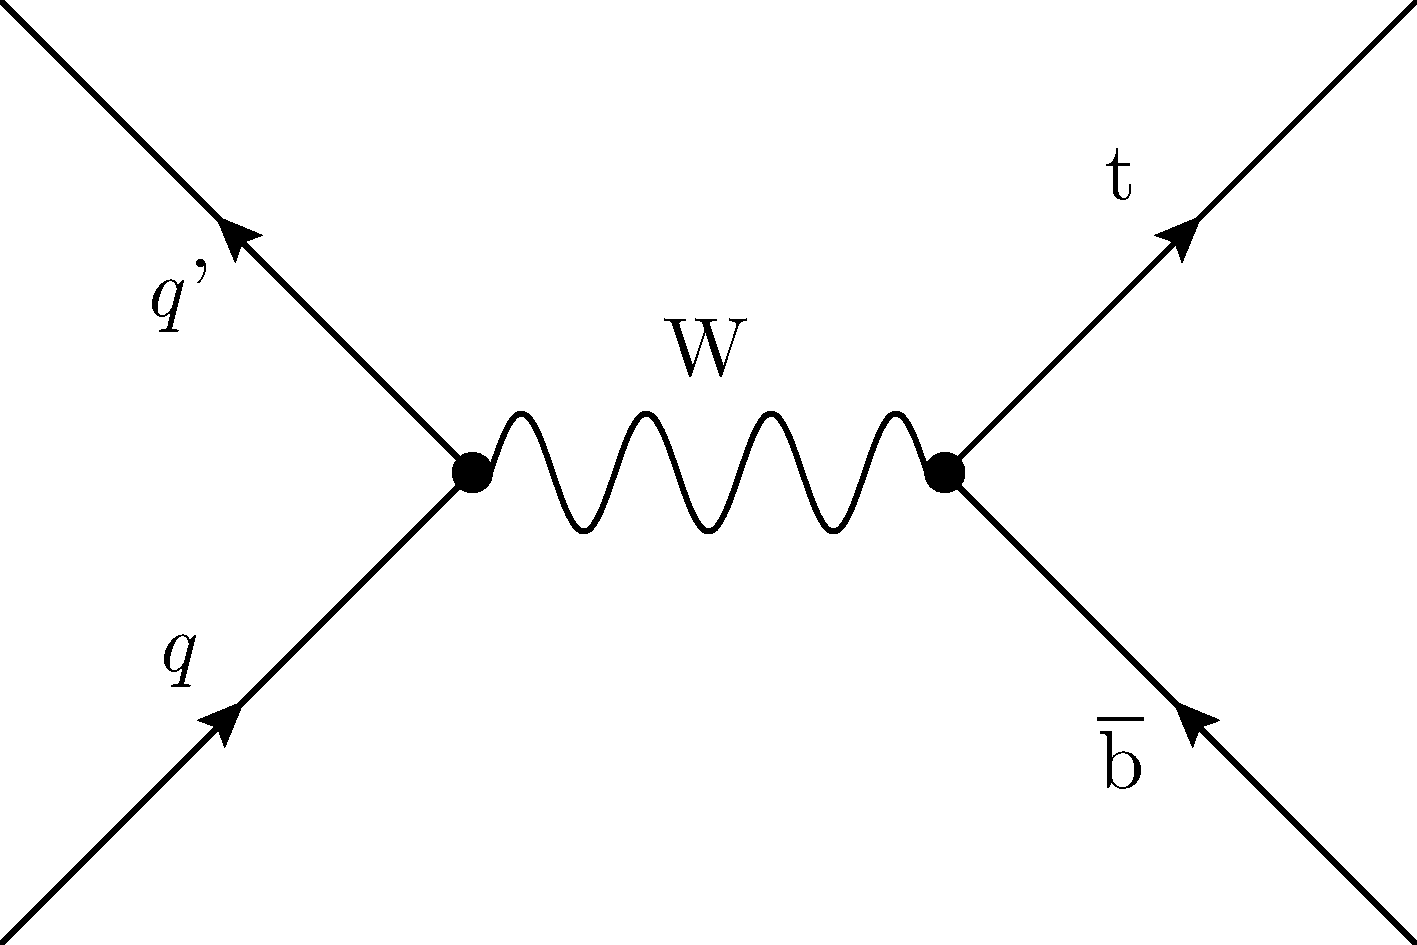
\includegraphics[width=\textwidth]{\figpath/FeynmanDiagramsPyFeyn/STopS.pdf}
    \caption{Production of a single top quark via the s-channel}
    \label{fig:STopS}
  \end{subfigure}
  \hspace{0.015\textwidth}
  \begin{subfigure}[t]{0.3\textwidth}
    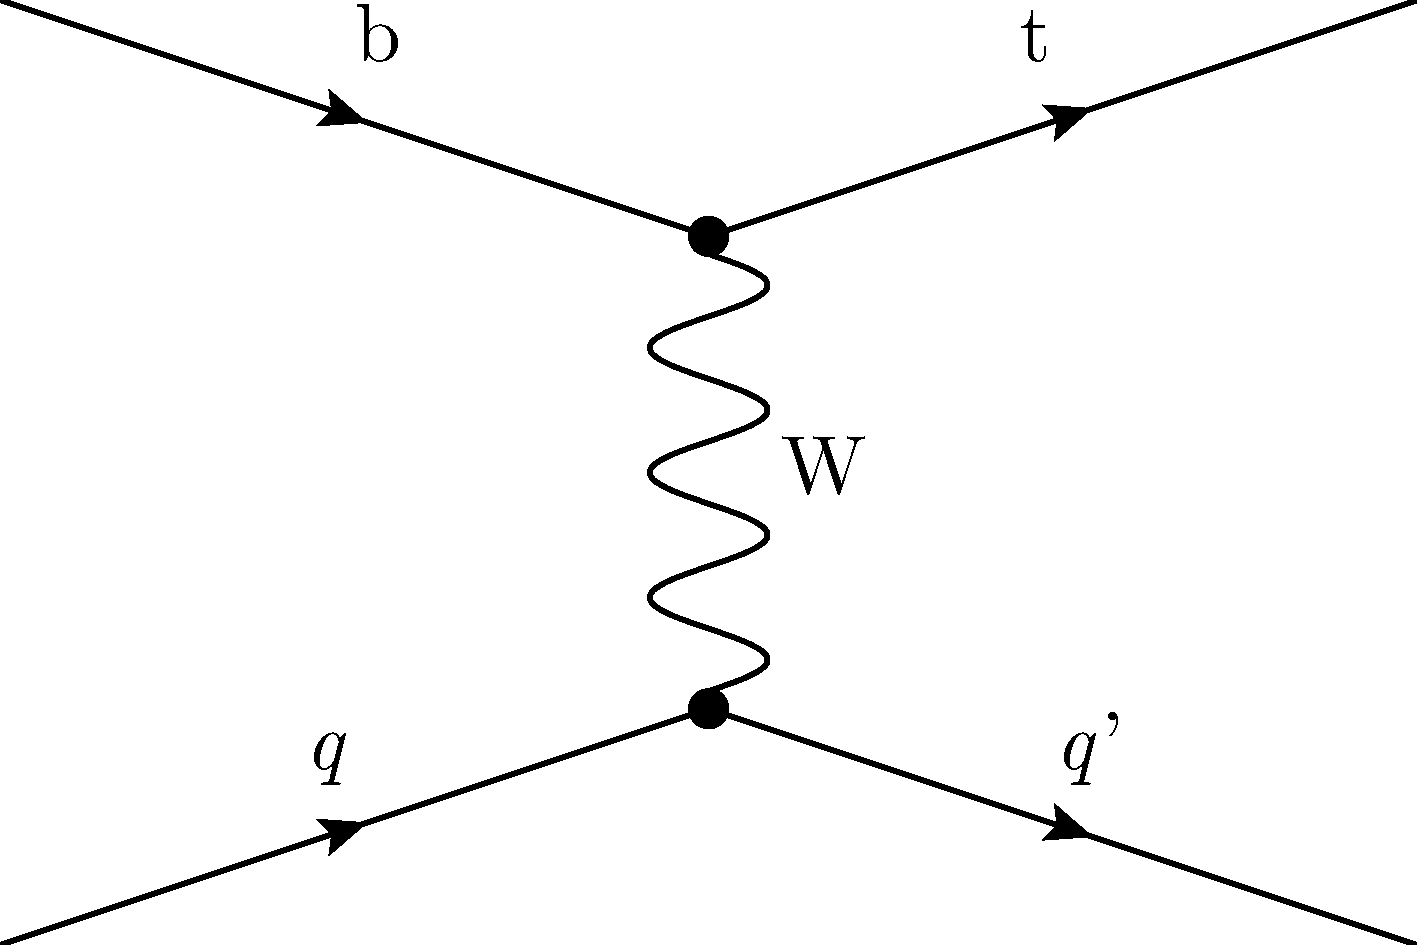
\includegraphics[width=\textwidth]{\figpath/FeynmanDiagramsPyFeyn/STopT.pdf}
    \caption{Production of a single top quark via the t-channel}
    \label{fig:STopT}
  \end{subfigure}
  \hspace{0.015\textwidth}
  \begin{subfigure}[t]{0.3\textwidth}
    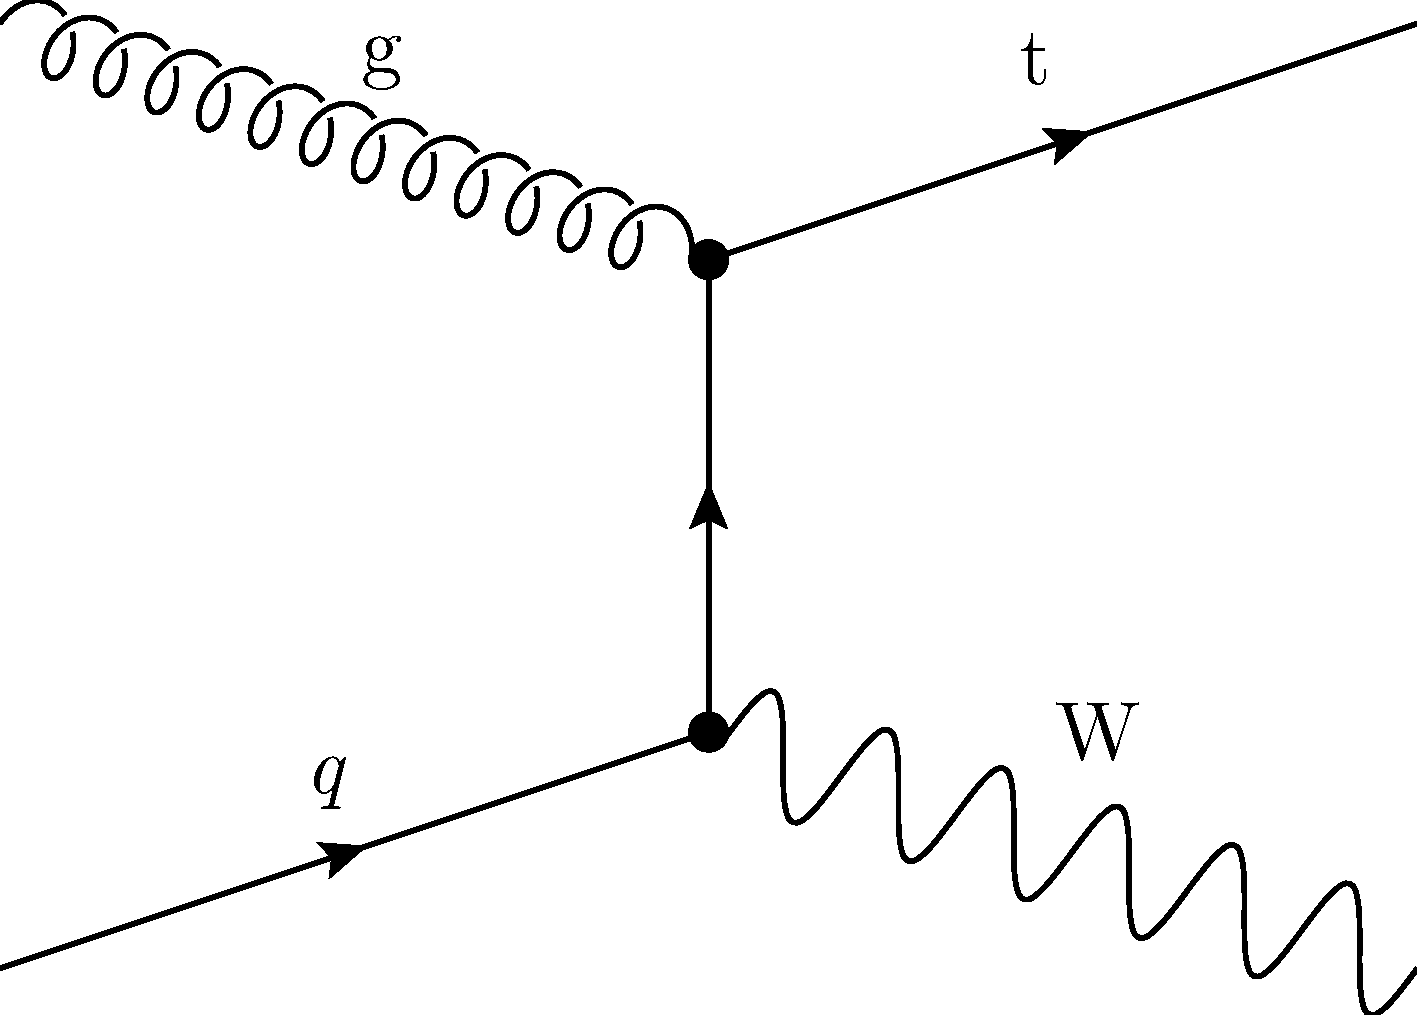
\includegraphics[width=\textwidth]{\figpath/FeynmanDiagramsPyFeyn/STopTW.pdf}
    \caption{Production of a single top quark via the tW-channel}
    \label{fig:STopTW}
  \end{subfigure}
  \caption{Example Feynman diagrams for the standard model single top processes. The final state particles are not pictured here.}
  \label{fig:SingleTopBackground}
\end{figure}

The backgrounds considered in this analysis are as follows:
\begin{itemize}
	\item \textbf{W$+$jets}: This is the production of a single \Wpm boson in association with final state quarks or gluons. If the \Wpm decays leptonically then the final state will match that of our signal. This process has an extremely high cross section and is thus the dominant background in the analysis.
	\item \textbf{Drell-Yan Z/$\gamma^{*}+$ jets}: In this case a \Z or $\gamma$ boson is produced in association with final state quarks or gluons. In order for this process to mimic the signal one lepton from the boson decay must be lost due to being outside the acceptance region or due to some reconstruction inefficiency. Although this process also has a high cross section, the requirement of having only one lepton reduces the prevalence of these processes in our signal region.
	\item \textbf{Diboson}: It is possible to mimic the final state signature with decays from several non-resonant diboson processes. The \WW process is an irreducible background as it can exactly mimic our signal. The \WZ process can produce the \lvqq final state in two ways: either the \W decays leptonically and the \Z decays hadronically or the \W decays hadronically and one of the leptons from the \Z decay is lost. The \ZZ process is similar in that one lepton from the leptonic \Z must be lost in order for the event to make it into the signal region.
	\item \textbf{\ttbar}: The tops will each decays to a \cPqb quark and a \W boson via the weak interaction. If the \W bosons decay semi-leptonically then the final state will be very similar, save for the presence of two additional b-quarks. If the b-jets can be identified then the events can be removed. Still, due to inefficiencies in identifying the b-quarks some \ttbar may still pass all selection requirements.
	\item \textbf{Single Top}: There are three production channels for this type of process: s-channel, t-channel, and the tW-channel. These processes have low cross sections and can produce reducible signatures.
	\item \textbf{Multi-jet}: This is the production of $n$ jets where one jet is mistakenly identified as a lepton and the jet energies are mis-reconstructed enough to produce a sufficient imbalance in the event to mimic the neutrino. While this might seem improbable, the QCD cross section is quite large and thus this become a non-negligible background for this analysis.
\end{itemize}
The Feynman diagrams for all of these backgrounds, except for QCD, can be found in figs.~\ref{fig:SingleBosonBackground},~\ref{fig:DibosonBackground},~\ref{fig:TTbarBackground}, and~\ref{fig:SingleTopBackground}.

\section{Beyond the Standard Model}
\label{sec:BSM}

While the standard model has been an incredibly successful theory (see appendix~\ref{appendix:standard_model_history}), it too has limitations.
These shortcoming manifest themselves as either observations which are not covered by SM or characteristics of SM for which there is no fundamental explanation.
In order to combat these shortcomings, a plethora of new theories have been created with the guiding principle that the new theories must be a superset of the standard model.
That is, they must be able to reproduce all of the SM observations that have been so thoroughly tested.
The following is a non-exhaustive list of shortcomings.
\begin{itemize}
	\item \textbf{Gravity} is not included as either a field or particle within the Standard Model. In addition, there is no explanation as to why gravity is a much weaker force when compared to the electroweak or strong forces. Nevertheless, we expect that quantum gravity effects will become important at the Planck scale, $m_{P}\sim10^{19}\gev$. There have been attempts to create supergravity theories~\cite{VANNIEUWENHUIZEN1981189,Freedman2012,Nastase:2011aa}, but these have not yet been unified with the rest of the Standard Model. Most of these theories include a particle called the graviton, which is the quantum of a spin-2 field.
	\item According to cosmological experiments such as Planck, the universe is made of only about 5\% ordinary, visible matter. Part of this remainder, about 26\%, is made of what is termed \textbf{dark matter} (DM)~\cite{Ade:2015xua,Clowe:2006eq}. We know that this gravitationally interacting substance must exist because of astrophysical measurements of galactic rotation curves and galaxy cluster collisions~\cite{Morrissey20121,Garrett:2010hd}. Still, the Standard Models does not provide any particle candidate.
	While the exact nature of DM is unknown, we do know that any DM particle must be stable, electrically neutral\footnote{The term ``dark'' comes from the fact that DM does not interact with photons and therefore is not visible to the human eye.}, weakly interacting, and a have a reasonably large mass. While this may sound like the SM neutrino, we already know that neutrino masses are too small~\cite{Bertone:2004pz}. This type of particle has been termed the WIMP or weakly interacting massive particle~\cite{Morrissey20121}, but other candidates have been proposed as well~\cite{PDG}.
	\item Besides visible and dark matter, the universe contains 69\% of something else which has been termed \textbf{dark energy} and is not included in the Standard Model. Scientists know very little about dark energy other than that it seems to be causing the acceleration of universal expansion, an action which could not come from any of the SM particles. Planck measurements indicate that dark energy is consistent with the theory of a cosmological constant. However, when there have been attempts to calculate the cosmological constant in terms of vacuum energy there have been mismatches of 100 orders of magnitude. 
	\item Physicists expect that equal amounts of \textbf{matter and antimatter} were created during the Big Bang. Nevertheless the visible universe is filled with matter, but contains very little antimatter. The Standard Model offers no explanation for this discrepancy unless some of the symmetries were violated (i.e. baryon number conservation, CP invariance, and C conservation)~\cite{0038-5670-34-5-A08,KUZMIN198536}.
	\item As explained in section~\ref{sec:higgs_mechanism}, Standard Model neutrinos are massless because they have no chiral right-handed counterparts and no Yukawa coupling with the scalar Higgs field. At the same time, there have been observations of \textbf{neutrinos oscillating} between flavors, which can only occur if at least two of the three neutrino types have mass~\cite{Abe:2008aa,Abe:2014ugx,Agafonova:2014ptn,Agashe:2014kda,PhysRevLett.81.1158}. To complicate matters, the physical neutrino eigenstates are mixtures of mass eigenstates $\left(\nu_{1},\nu_{2},\nu_{3}\right)$, which cannot be measured directly. There have been no direct measurements of the neutrino masses to date, but there have been upper limits placed on the masses and the squared mass differences are known.
	\item Studies of the Z boson have shown that no fourth generation of fermions with light neutrinos exists~\cite{DECAMP1990399}. However, there is nothing in the Standard Model which forbids a \textbf{fourth generation}. Could there be a fourth family of fermions with heavy neutrinos?
	\item Is there a reason for the Standard Model fermion couplings to the Higgs boson? In other words, why do the fermion masses vary over five orders of magnitude from 0.511\mev for the electron to 173\gev for the top quark? This is sometimes called the \textbf{fermion mass hierarchy problem}.
	\item \textbf{Baryon and lepton conservation} are accidental symmetries without enforcement by a local gauge symmetry. Are these really conserved quantities?
	\item Why is the $\mu^{2}$ from the Higgs potential negative? It needs to be negative to ensure EWSB, but there is no other compelling reason.
	\item We know that there are different mass scales in the universe. The Standard Model is effective at the electroweak scale of $\mathcal{O}\left(\mathrm{100}\gev\right)$. However, at the Planck scale, $\mathcal{O}\left(\mathrm{10^{19}}\gev\right)$, the model starts to break down and requires quantum gravity effects to be valid. As a consequence of the different scales, the bare parameters of the SM can differ from their renormalized values by several orders of magnitude. This in and of itself will not invalidate the model, but one would need to accept some amount of ``fine tuning''. These types of problems are called ``hierarchy problems''. There is one problem in particular, however, which is known colloquially as \textbf{the hierarchy problem}. Observed particle masses are a combination of the ``bare'' mass at tree level and the radiative corrections from loop diagrams. The problem comes from loop corrections to the Higgs mass parameter $\mu=m_{h}/\sqrt{2}$ introduced in section~\ref{sec:higgs_mechanism}. The Higgs mass can be written in terms of the bare mass parameter $\mu_{0}$ and radiative corrections $\delta\mu$
		\begin{equation}
			\mu^{2}=\mu_{0}^{2}+\delta\mu^{2}
		\end{equation}
	The largest correction comes from the one-loop diagrams dealing with the top quark, the heaviest particle in the Standard Model. The one loop corrections to Higgs are shown in fig~\ref{fig:one_loop_corrections_to_higgs_mass}. While fermions and bosons are protected from these divergences, scalars like the Higgs have a large dependence on the ultraviolet (UV) cutoff. This means that while the observed Higgs mass is $\sim\textrm{125}\gev$, radiative corrections should drive $\mu^{2}$ and thus the mass up to very large values. If the bare mass and radiative corrections happened to cancel at such a precise level as to lead to the observed mass it would be and \textit{unnatural} amount of fine tuning~\cite{SUSSKIND1984181}. Fine tuning problems like this have traditionally been interpreted as the existence of new physics~\cite{Morrissey20121}.
\end{itemize}
\begin{figure}[hbt]
    \centering
    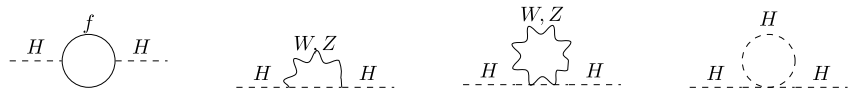
\includegraphics[width=0.95\textwidth]{\figpath/Chapter2/OneLoopCorrectionsToHiggsMass.png}
    \caption{Feynman diagrams for the one-loop corrections to the Higgs boson mass. From left to right: contribution from the Yukawa interaction; two contributions from the gauge interaction; contribution from the Higgs self-interaction.}
    \label{fig:one_loop_corrections_to_higgs_mass}
\end{figure}

In order to answer the open questions or provide a more complete theory, there have been numerous models of beyond-the-SM (BSM) physics developed. While some of these models are still being tested by the LHC and other experiments, some previous BSM models were ruled out by Higgs discovery~\cite{Cheng:2007bu}. Below I list a small selection of BSM models which have been proposed as extensions to the SM.
\begin{itemize}
	\item There are a whole host of little Higgs theories proposed~\cite{Cheng:2007bu,Reuter:2012sd,Schmaltz:2005ky}. In these models the Higgs boson is seen as the pseudo-Goldstone boson of a global symmetry broken around 10\tev. In addition to the current array of SM particles, a little Higgs model would include new particles with the same spin as the SM particles. An additional symmetry called T-parity would be introduced, which says that particles must be introduced in pairs. This implies that the additions to the SM would only impact observables at the loop-level.
	\item Models of extra spatial dimensions say that the electroweak scale is the only fundamentally short distance scale and that loop corrections to the Higgs mass cut off at the electroweak scale and not the Planck scale~\cite{ArkaniHamed:1998rs}. The reduction in the cutoff scale leads to less fine tuning. A key feature of these models is that gravity, but not the other gauge interactions, permeates the new dimensions, which is why it is seen as being much weaker than the other forces. The Planck scale in $\left(4+n\right)$ dimensions is assumed to be on the order of the electroweak scale. For $n\geq2$ the size of the new dimensions is sub-millimeter, which is a scale where gravity has not been thoroughly tested.
	\item Supersymmetry (SUSY) was first proposed by Miyazawa in 1966 in order to relate mesons and baryons for hadronic physics~\cite{doi:10.1143/PTP.36.1266,PhysRev.170.1586}. In the 1970s it was rediscovered as a QFT by several groups. In short SUSY introduces a new space-time symmetry that relates fermions to bosons and immediately provides a solution to the hierarchy problem~\cite{WESS197439,Golfand:1971iw,PhysRevLett.49.970,PhysRevD.49.6173,FAYET1975104,BARBIERI1982343,PhysRevD.27.2359,Martin:1997ns}. Each SM particle has a SUSY partner that differs in spin by 1/2. The coupling of the particles are chosen so that the Higgs mass does not diverge due to loop corrections. Additionally, SUSY causes EWSB in a different way that does not require negative $\mu^{2}$, answering another question left by the SM. Although SUSY models can cause protons to decay, many introduce R-parity to prevent this. If R-parity conserved then the lightest supersymmetric particle (LSP) is stable (i.e. the LSP can't decay without violating R-parity). SUSY is a appealing model because the LSP also provides a DM candidate as the particle would be heavy and weakly interacting. While the theory has significant promise, SUSY has not yet been observed. This however, does not mean that SUSY is wrong. It simply means that the masses of the supersymmetric partners are not the same as their SM partners (i.e. SUSY is broken somehow).
\end{itemize}

